\chapter{Phase 3: Hardening \& Mitigation}

This chapter presents the Blue Team response to the vulnerabilities identified and exploited in the previous phases. The objective is to implement a set of countermeasures that enforce the three fundamental security properties — \textbf{integrity}, \textbf{confidentiality}, and \textbf{authenticity} — on the same resource-constrained ESP8266 hardware.

\medskip
\noindent Unlike Phase~2, where the malicious firmware was developed using the Mongoose OS framework to match the original Shelly ecosystem, the hardened firmware for Phase~3 was built entirely using the \textbf{Arduino IDE} (with the ESP8266 Arduino Core). This deliberate choice was made to vary the development approach and to demonstrate that the same hardware can be programmed using different toolchains. The Arduino ecosystem also provides direct access to the \textbf{BearSSL} cryptographic library, which is essential for implementing both TLS-based MQTT communication and RSA-based firmware signature verification within the tight memory constraints of the ESP8266.

\medskip
\noindent The hardened firmware (\texttt{ShellyPlugS.ino}) preserves the same functional capabilities as the Phase~2 variant — relay control, energy monitoring via the HLW8012, MQTT telemetry publishing, and an embedded web interface (Figure~\ref{fig:bluefw_ui}) — but introduces two critical security layers:

\begin{enumerate}
    \item \textbf{Secure OTA Update with Firmware Signing}: Cryptographic signing of firmware binaries using RSA-2048 and verification of the digital signature before applying any update, preventing the injection of unauthorized code (Section~\ref{sec:integrity}).
    
    \item \textbf{Secure MQTT Communication with mTLS}: Migration from plaintext MQTT (port 1883) to MQTTS (port 8883) using TLS 1.2 with mutual authentication via X.509 certificates, preventing eavesdropping and unauthorized broker/client impersonation (Section~\ref{sec:confidentiality}).
\end{enumerate}

\begin{figure}[H]
    \centering
    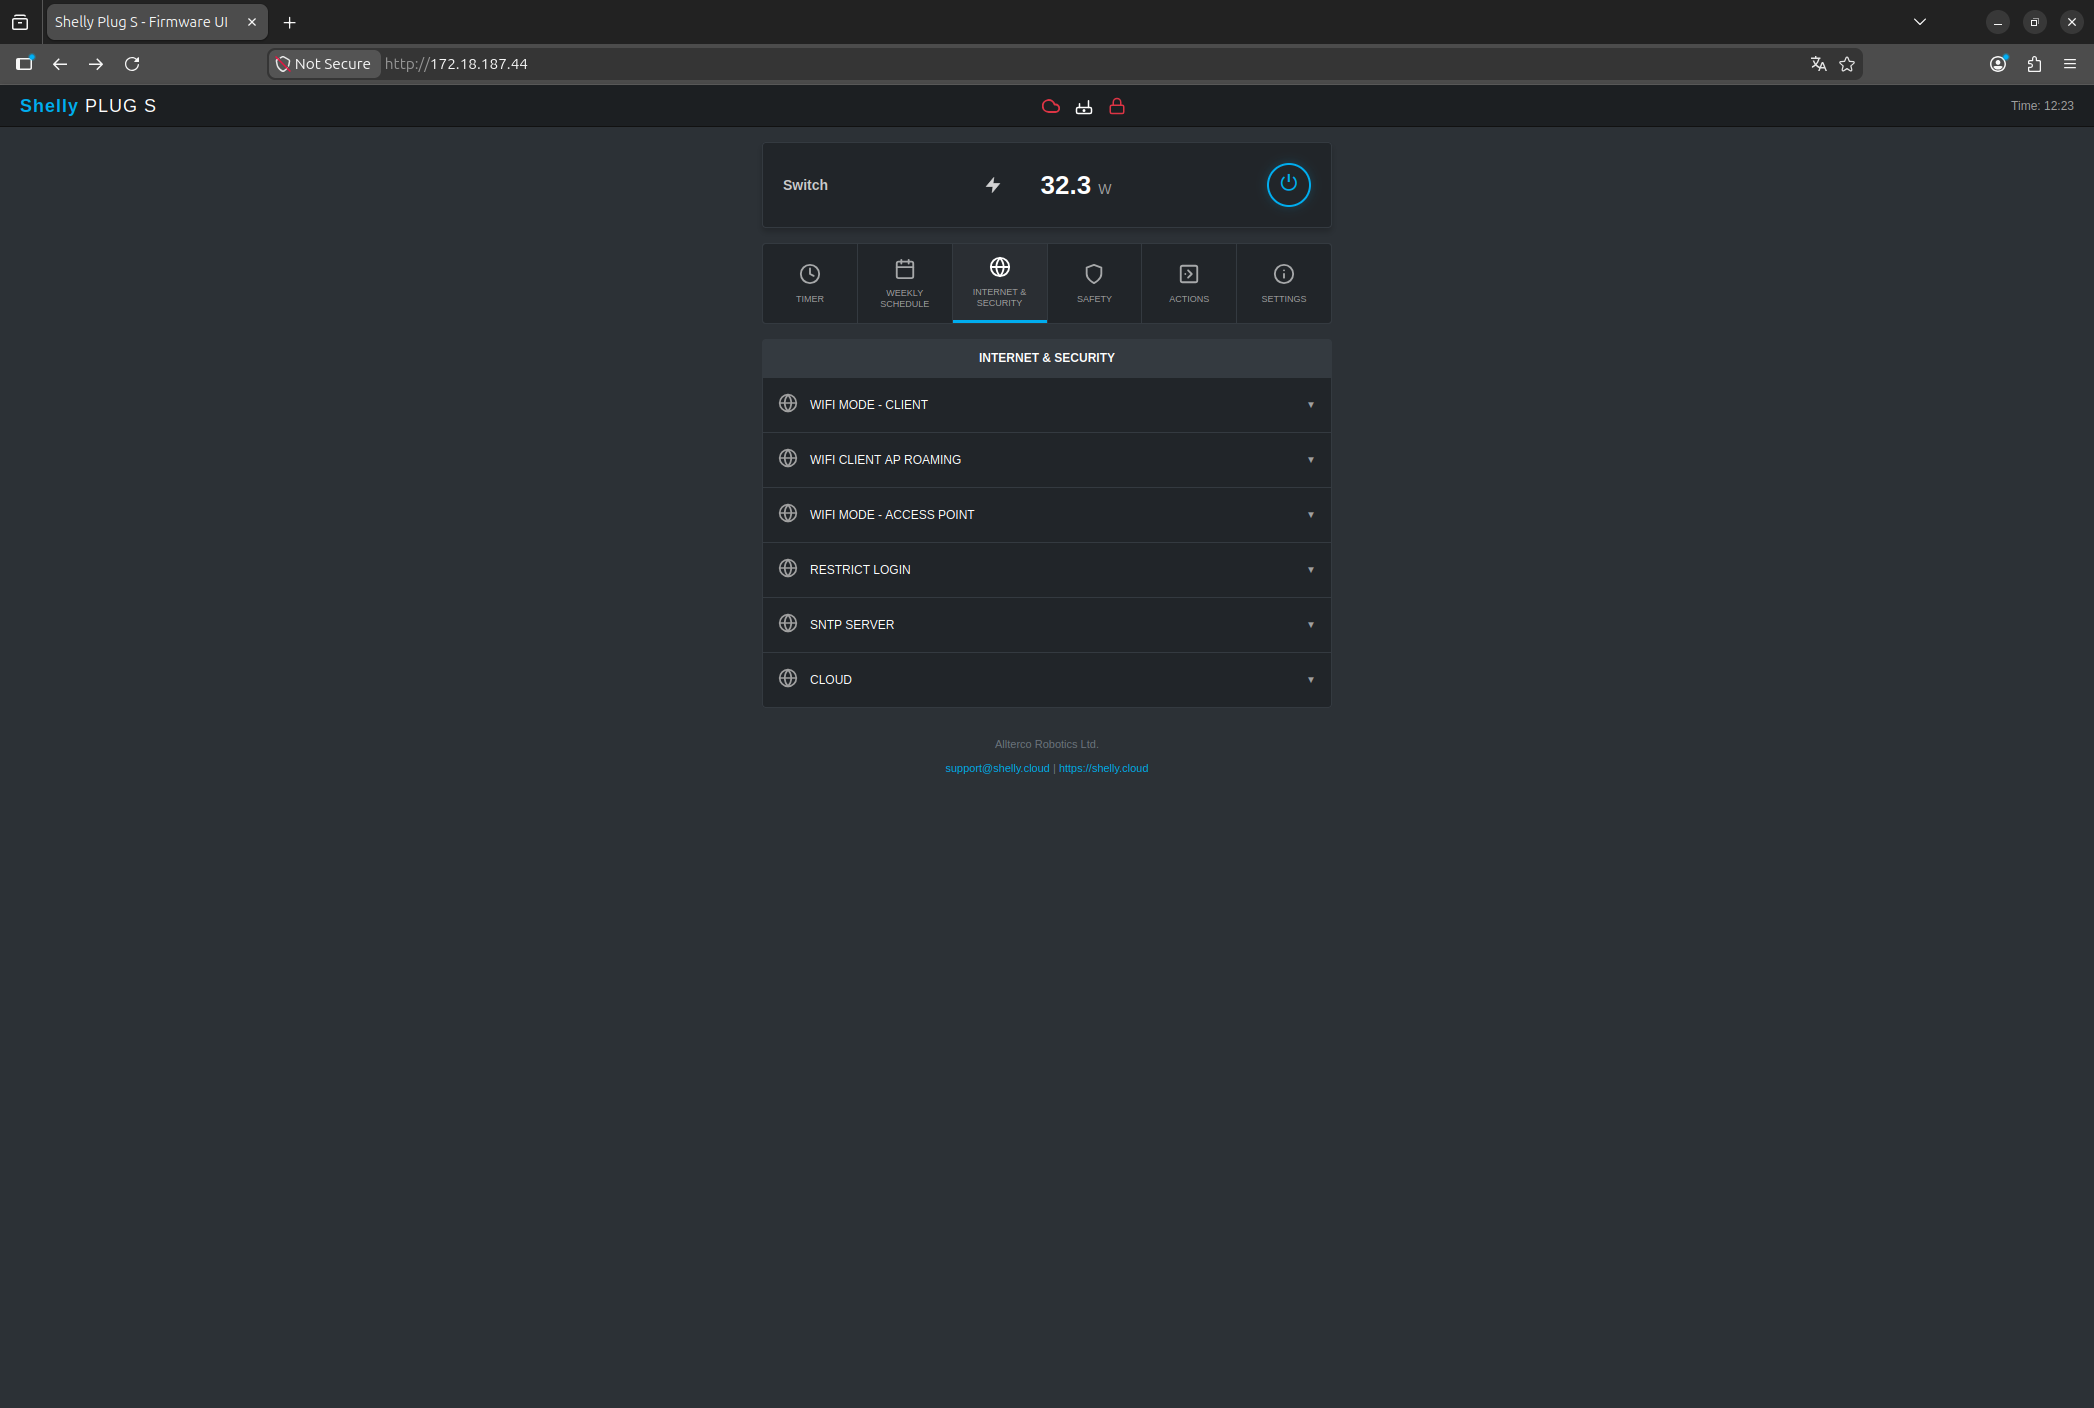
\includegraphics[width=0.90\linewidth]{Images/Fase3/InterfacciaBlufw.png}
    \caption{Web interface of the hardened firmware, preserving the same look and feel as the original Shelly UI while adding secure OTA update capabilities}
    \label{fig:bluefw_ui}
\end{figure}


\section{Ensuring Integrity: Secure Update Implementation}
\label{sec:integrity}

The most critical vulnerability exploited in Phase~2 was the \textbf{complete absence of cryptographic verification} during the OTA update process. The original Shelly firmware accepted any binary from any source — whether via the \texttt{/ota} endpoint or through a MITM-hijacked update flow — without verifying its authenticity or integrity. This section describes the countermeasure implemented to address this vulnerability: a \textbf{digital signature scheme based on RSA-2048 with SHA-256 hashing}, using the PKCS\#1 v1.5 padding scheme.

\medskip
\noindent The approach follows a standard asymmetric cryptography model:
\begin{itemize}
    \item The firmware developer signs each binary \textbf{offline} using a private key that never leaves the build environment.
    \item The device embeds the corresponding \textbf{public key} in its flash memory and uses it to verify the signature of any uploaded binary \textbf{before} applying the update.
\end{itemize}

\noindent This ensures that only firmware produced by the legitimate developer — who possesses the private key — can be installed on the device. Any attempt to upload unsigned or tampered binaries is rejected.

\subsection{Firmware Signing}

The signing process is performed offline on the developer's machine using two Python scripts: \texttt{key.py} for RSA key pair generation, and \texttt{signature.py} for computing and appending the digital signature to the firmware binary.

\subsubsection{Key Pair Generation}

The first step is generating the RSA-2048 key pair. The script \texttt{key.py} (Figure~\ref{fig:key_gen}) uses the \texttt{cryptography} Python library to generate a 2048-bit RSA key pair with a public exponent of 65537 (a standard and secure choice). The private key is saved in PEM format (PKCS\#8, unencrypted) to \texttt{private\_key.pem}, while the public key is exported in \texttt{SubjectPublicKeyInfo} format to \texttt{public\_key.pem}.

\begin{figure}[H]
    \centering
    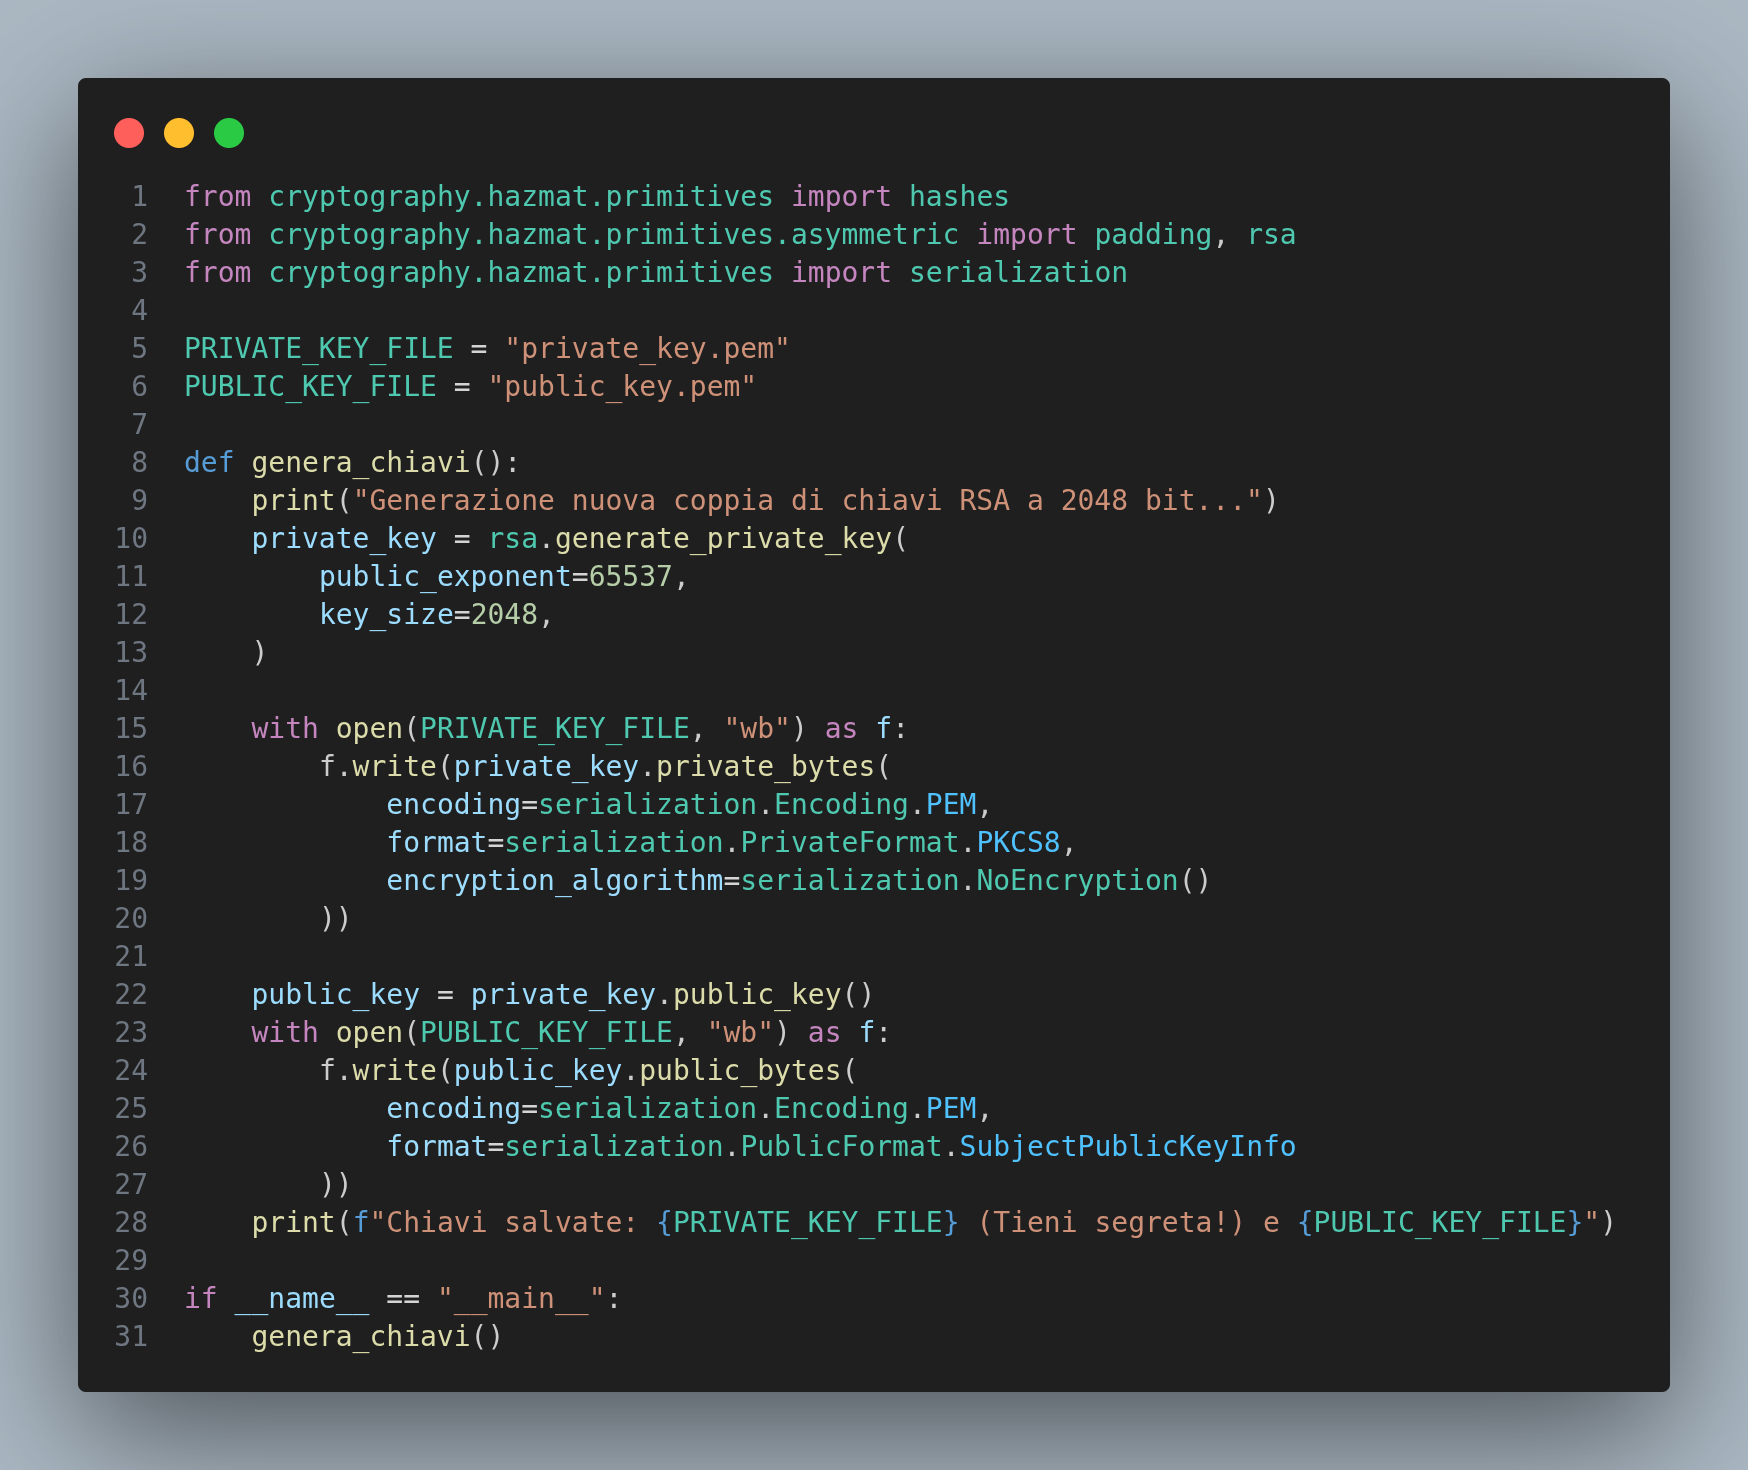
\includegraphics[width=0.80\linewidth]{Images/Fase3/GenerazioniChiaviFirma.png}
    \caption{RSA-2048 key pair generation script (\texttt{key.py}): generates \texttt{private\_key.pem} (kept secret) and \texttt{public\_key.pem} (embedded in firmware)}
    \label{fig:key_gen}
\end{figure}

\noindent The key generation is executed with:

\begin{bashcode}
python key.py
\end{bashcode}

\noindent This produces two files:
\begin{itemize}
    \item \texttt{private\_key.pem} — Must be kept secret and stored securely; it is used exclusively during the signing process on the developer's machine.
    \item \texttt{public\_key.pem} — Embedded directly into the firmware source code (in the \texttt{public\_key\_pem[]} constant) and flashed onto the device.
\end{itemize}


\subsubsection{Signing Process}

Once the firmware is compiled using Arduino IDE (producing a \texttt{.bin} file), it is signed using the \texttt{signature.py} script (Figure~\ref{fig:firma_fw}). The signing process operates as follows:

\begin{enumerate}
    \item \textbf{Read} the entire firmware binary into memory.
    \item \textbf{Compute} the SHA-256 hash of the binary data.
    \item \textbf{Sign} the hash using the RSA-2048 private key with PKCS\#1 v1.5 padding, producing a 256-byte digital signature.
    \item \textbf{Construct} the signed binary by appending to the original firmware data:
    \begin{itemize}
        \item The 256-byte RSA signature.
        \item A 4-byte little-endian integer encoding the signature length (i.e., \texttt{0x00000100} = 256).
    \end{itemize}
\end{enumerate}

\begin{figure}[H]
    \centering
    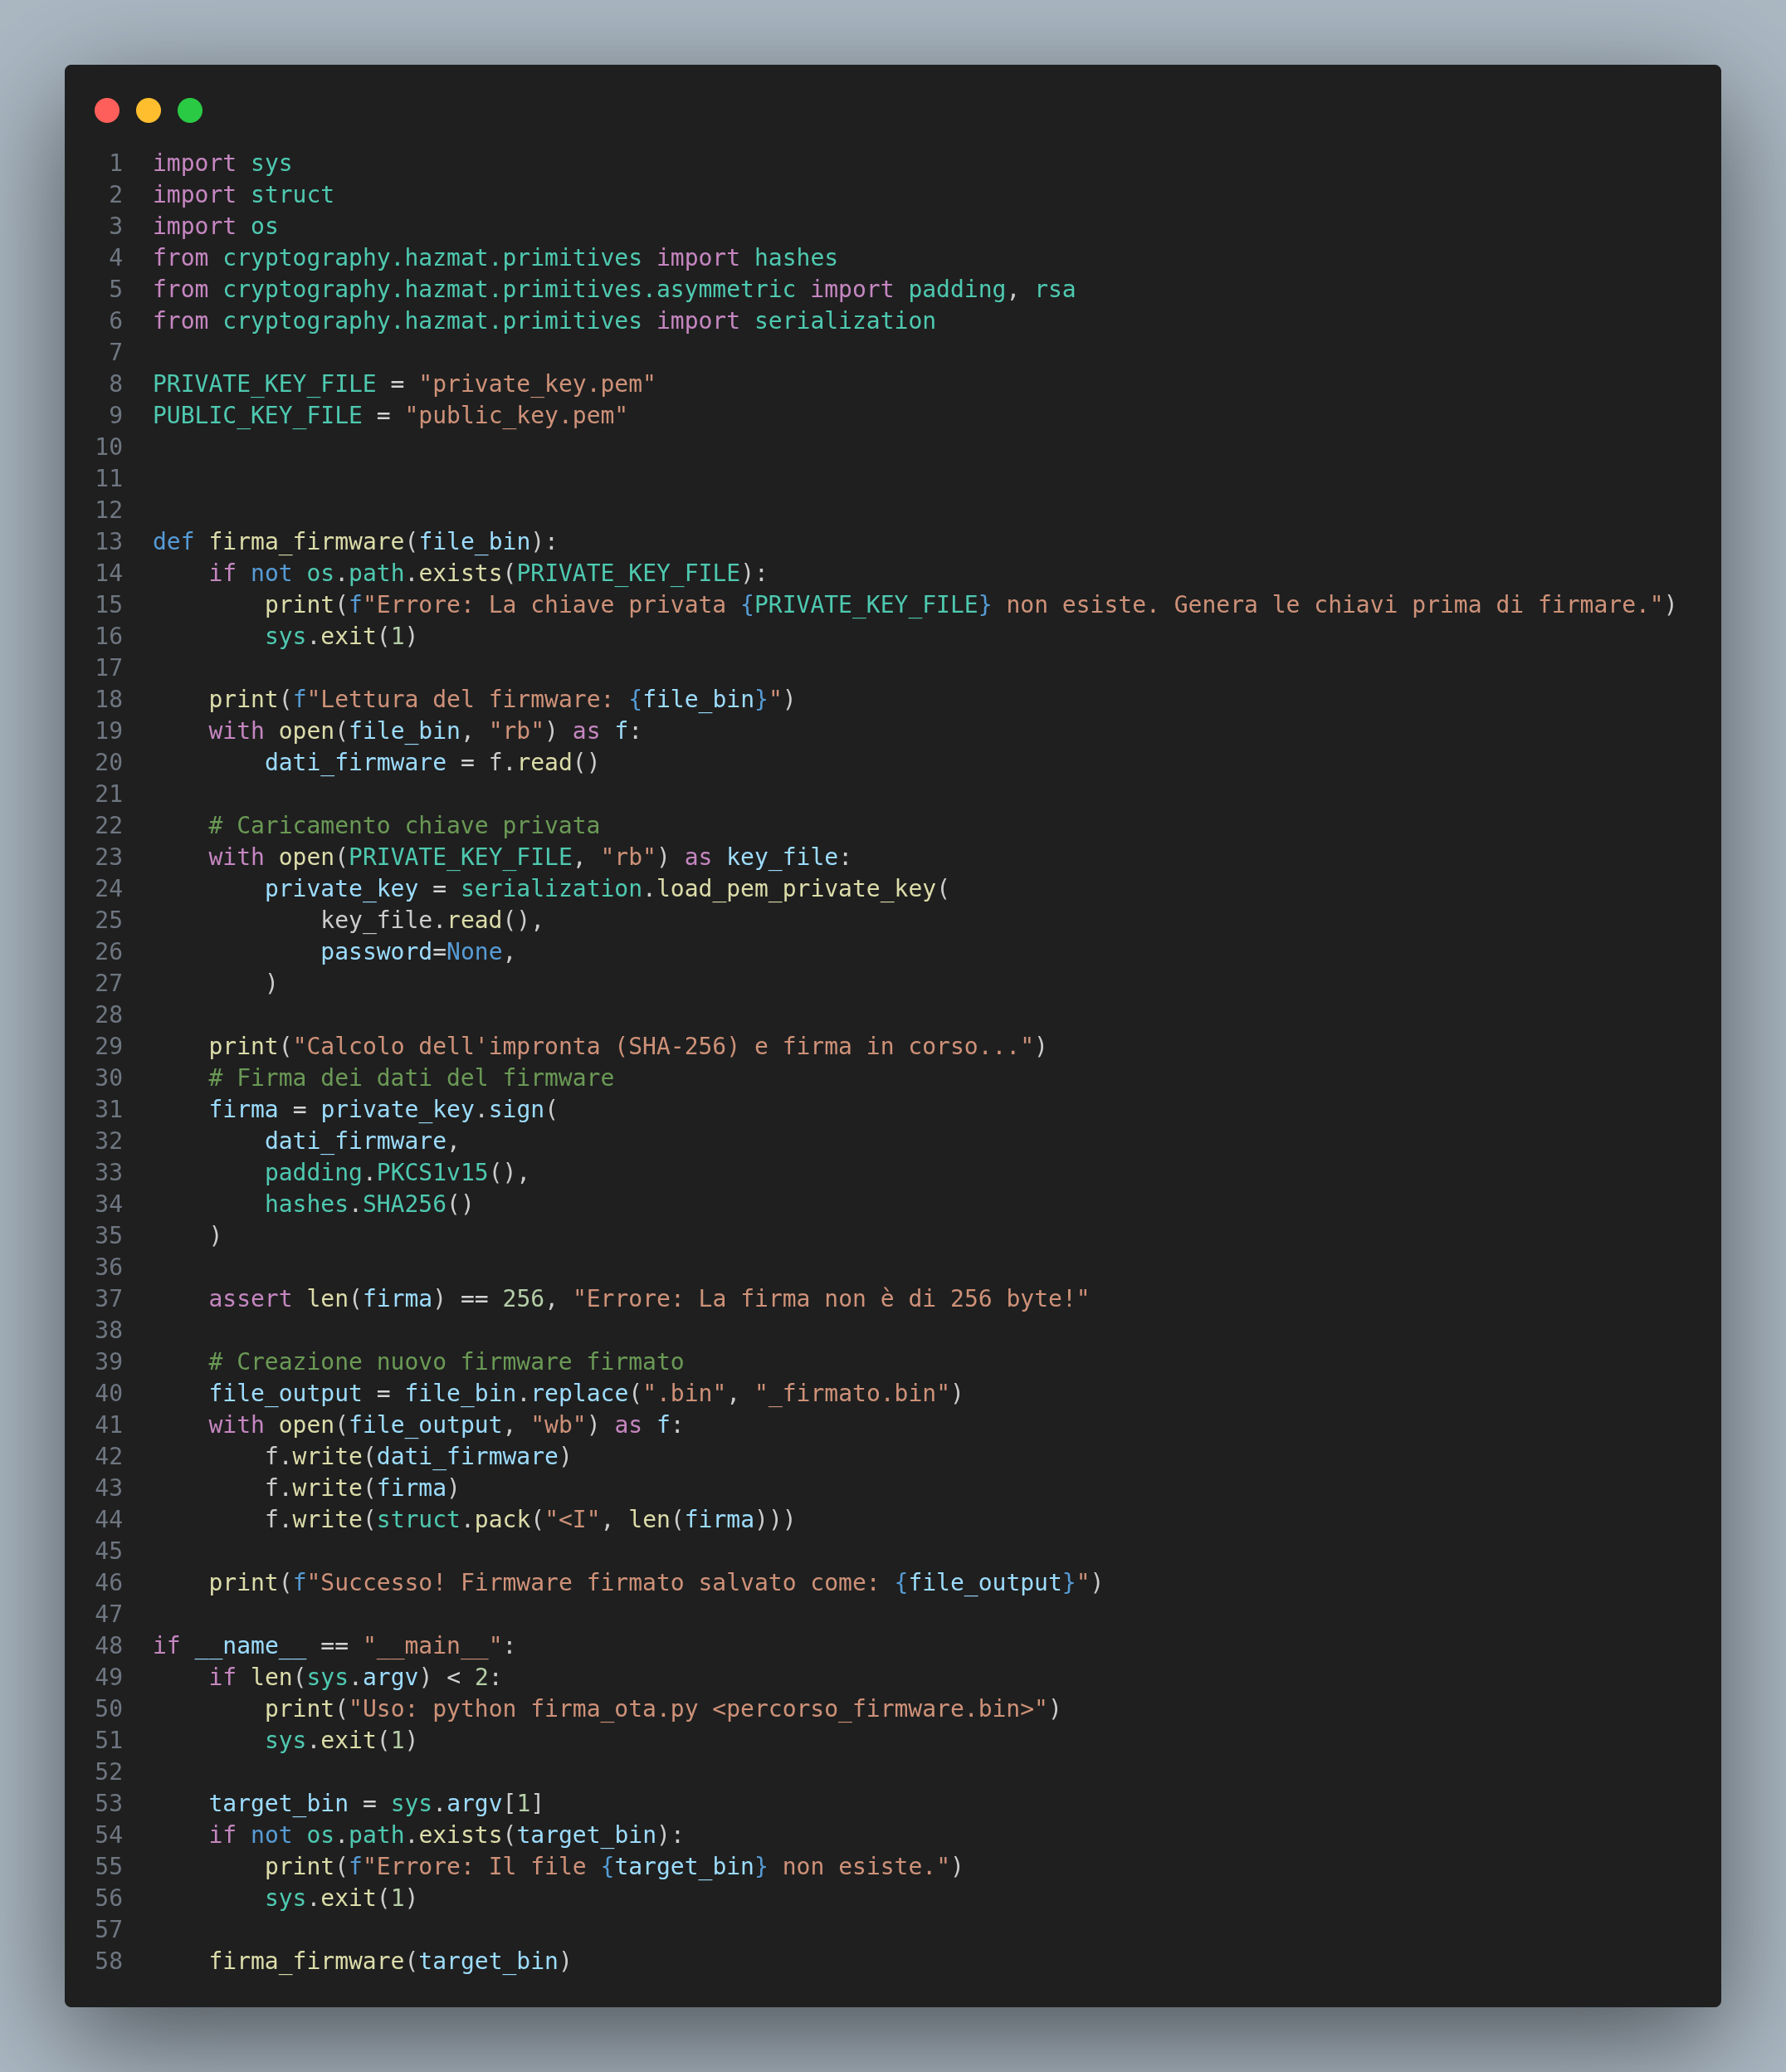
\includegraphics[width=0.80\linewidth]{Images/Fase3/firmaFirmware.png}
    \caption{Firmware signing script (\texttt{signature.py}): computes SHA-256 hash, signs with RSA-2048 PKCS\#1 v1.5, and appends the signature to the binary}
    \label{fig:firma_fw}
\end{figure}

\noindent The signing is executed with:

\begin{bashcode}
python signature.py ShellyPlugS.ino.bin
\end{bashcode}

\noindent This produces a signed binary named \texttt{ShellyPlugS.ino\_firmato.bin} with the following internal structure:

\begin{verbatim}
+-----------------------------+
| Original firmware binary    |   (N bytes)
+-----------------------------+
| RSA-2048 signature          |   (256 bytes)
+-----------------------------+
| Signature length (LE uint32)|   (4 bytes, value = 256)
+-----------------------------+
\end{verbatim}

\noindent The trailing 4-byte length field allows the device to locate and extract the signature from the end of the uploaded file during verification.


\subsection{Signing Verification}

The verification process occurs \textbf{on the device} during the OTA upload. The hardened firmware embeds the RSA-2048 public key directly in flash memory (stored in the \texttt{PROGMEM} section to minimize RAM usage) and uses the BearSSL library to perform signature verification before applying any update.

\subsubsection{Public Key Embedding}

The public key corresponding to the signing private key is hardcoded into the firmware source as a PEM-encoded string constant (Figure~\ref{fig:chiavi}):

\begin{figure}[H]
    \centering
    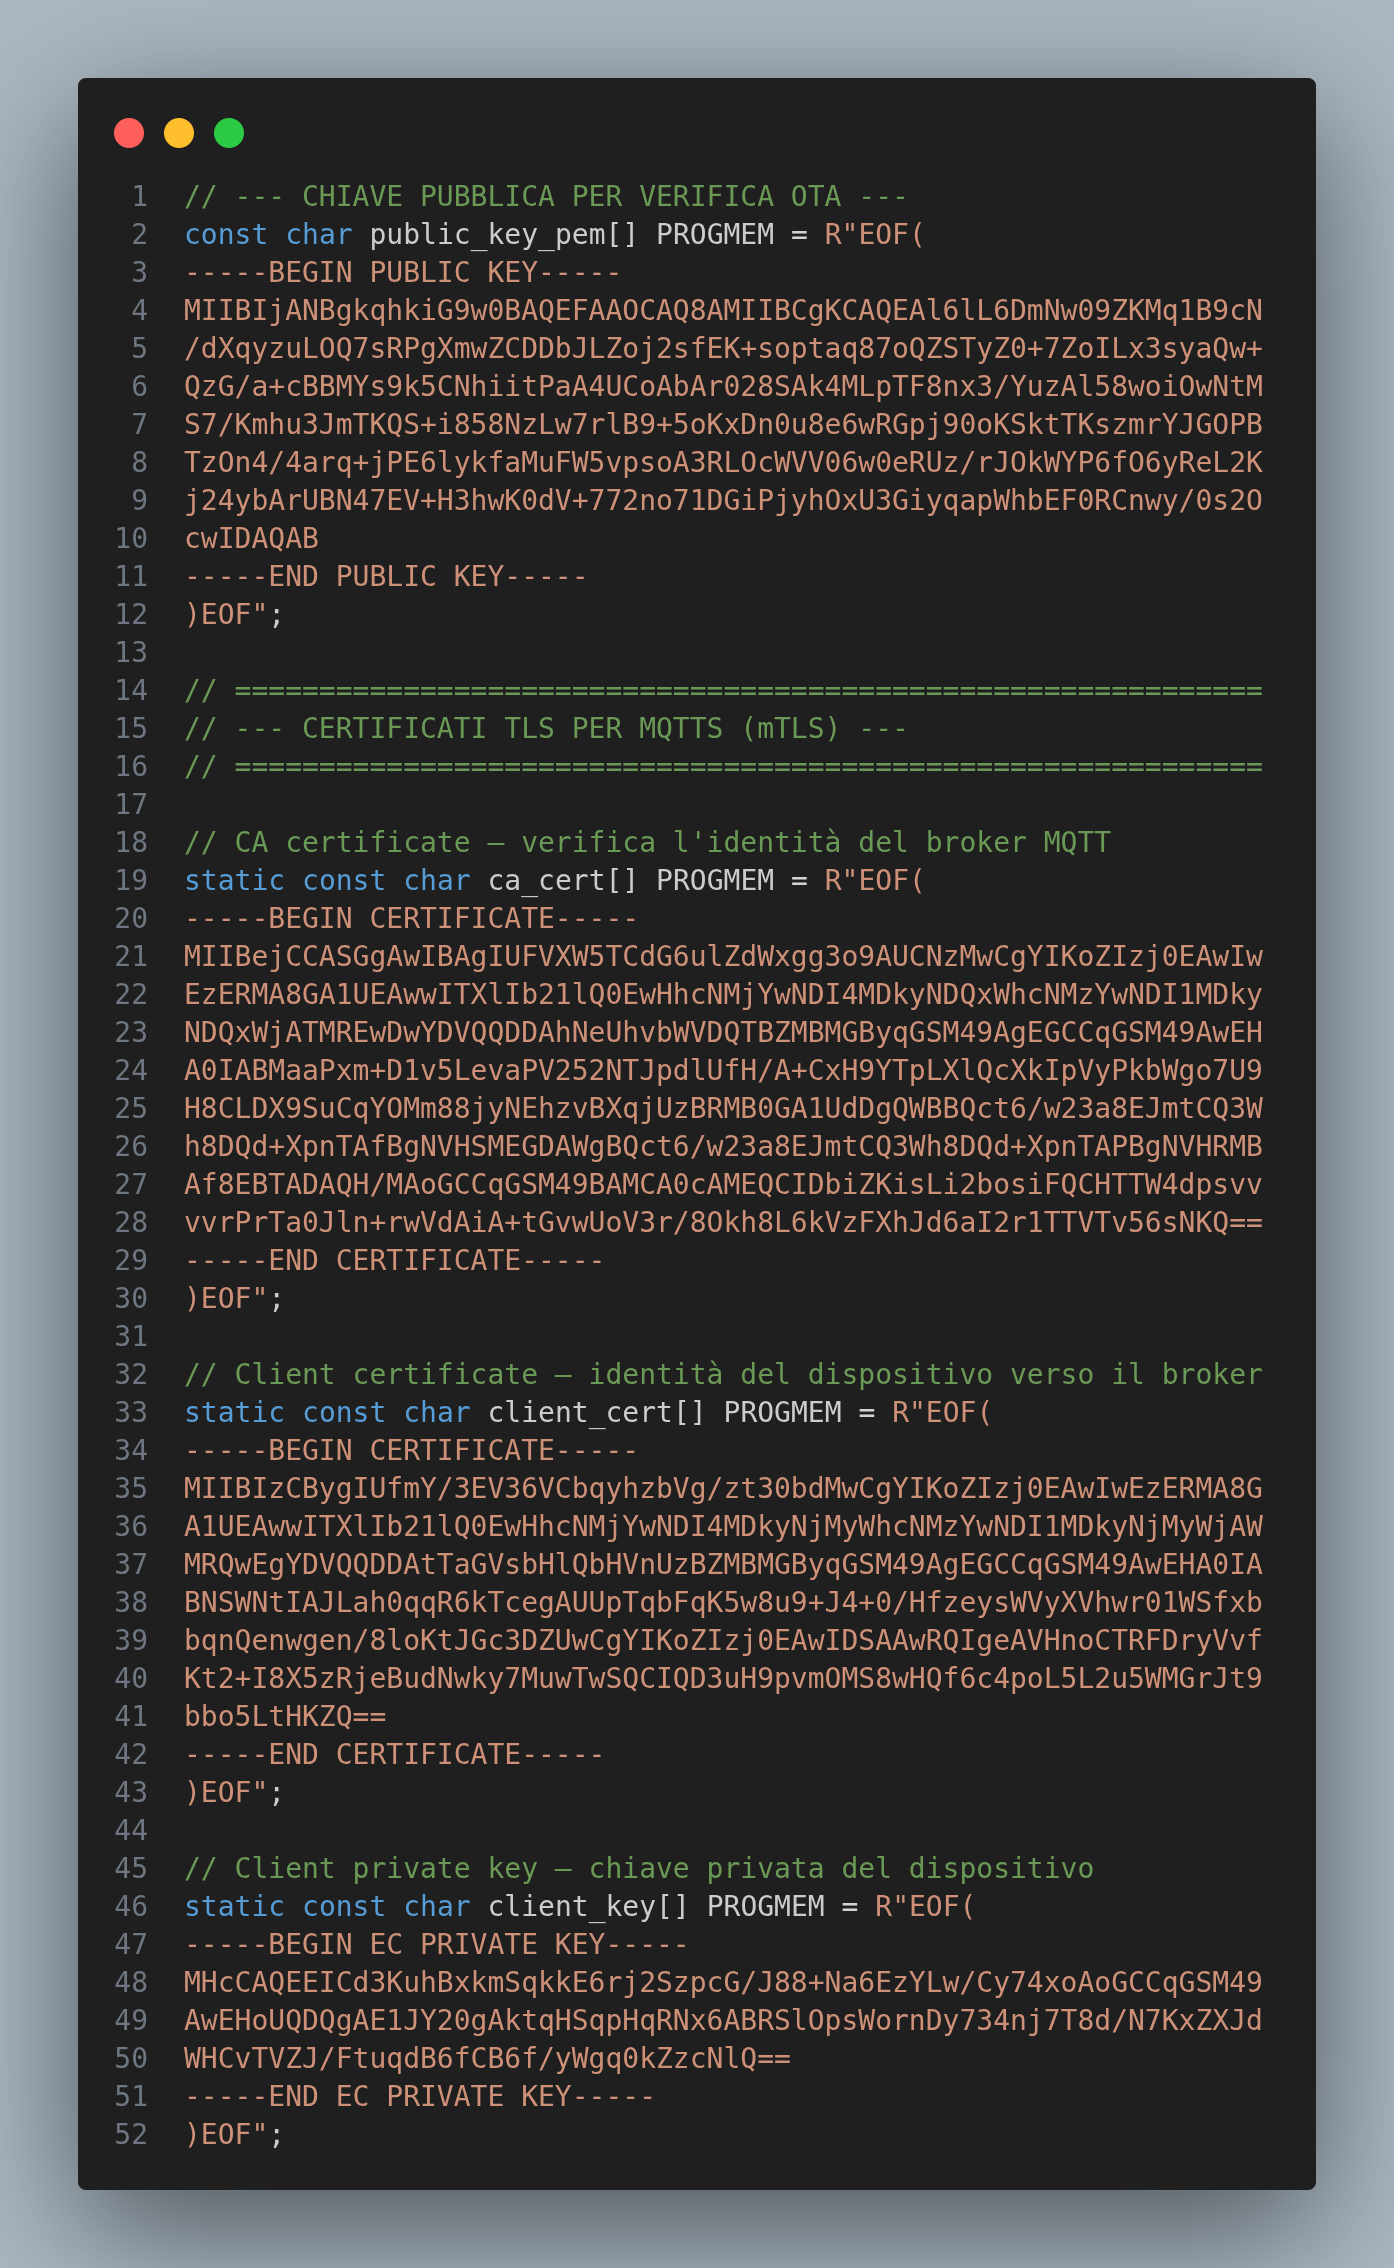
\includegraphics[width=0.80\linewidth]{Images/Fase3/chiavi.png}
    \caption{Public key for OTA verification and TLS certificates for MQTTS, all embedded in the firmware source code as \texttt{PROGMEM} constants}
    \label{fig:chiavi}
\end{figure}

\noindent The public key is stored in the \texttt{public\_key\_pem[]} array using the \texttt{PROGMEM} attribute, which instructs the ESP8266 compiler to place the data in flash memory rather than SRAM, preserving the limited heap space available for runtime operations.

\subsubsection{Verification Handler}

The OTA update endpoint (\texttt{/update}) has been completely redesigned compared to the original Shelly firmware. Instead of blindly accepting any uploaded binary, the hardened firmware implements a \textbf{three-phase upload handler} (Figure~\ref{fig:verifica_firma}) that performs cryptographic verification using BearSSL:

\begin{figure}[H]
    \centering
    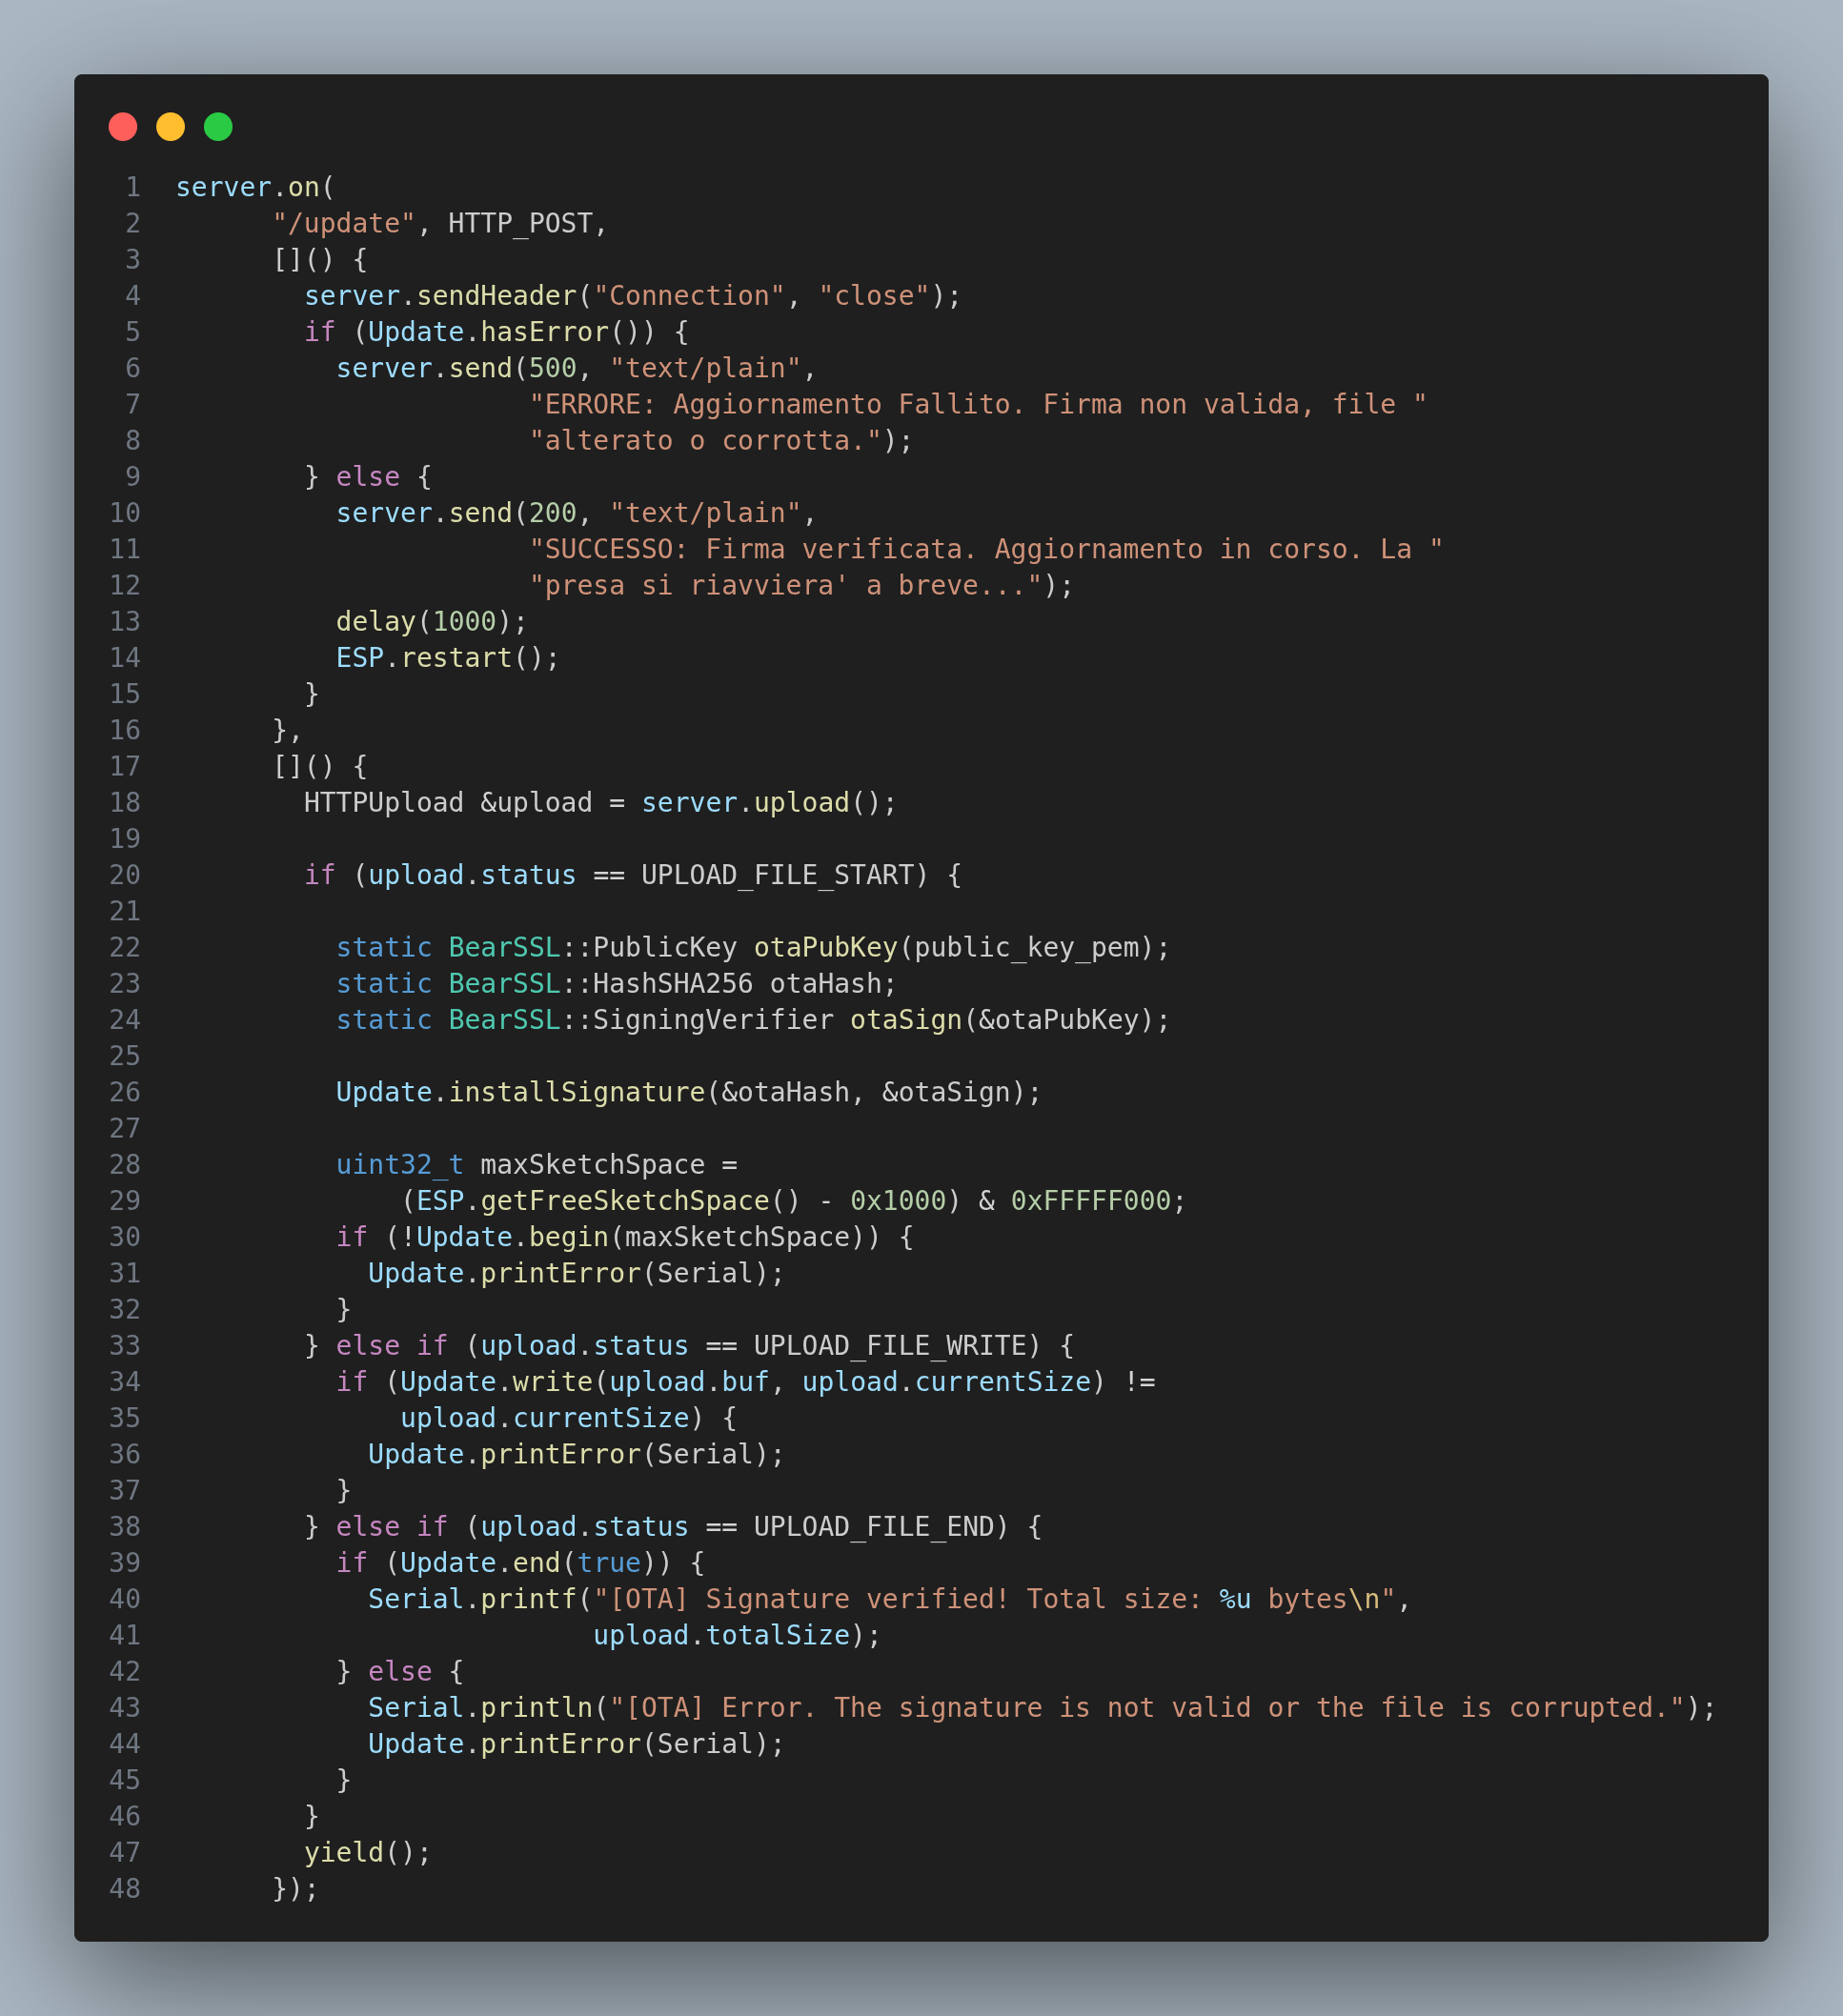
\includegraphics[width=0.80\linewidth]{Images/Fase3/codiceVerificaFirmaUpdate.png}
    \caption{OTA signature verification handler: BearSSL-based RSA-2048/SHA-256 verification integrated into the ESP8266 \texttt{Update} library}
    \label{fig:verifica_firma}
\end{figure}

\noindent The verification logic operates across three upload phases:

\begin{enumerate}
    \item \textbf{\texttt{UPLOAD\_FILE\_START}}: When the upload begins, the handler initializes the BearSSL verification pipeline:
    \begin{itemize}
        \item A \texttt{BearSSL::PublicKey} object is created from the embedded PEM public key.
        \item A \texttt{BearSSL::HashSHA256} object is instantiated for computing the firmware hash.
        \item A \texttt{BearSSL::SigningVerifier} object links the public key to the hash engine.
        \item The \texttt{Update.installSignature()} method registers the hash and verifier with the ESP8266 \texttt{Update} library.
    \end{itemize}
    
    The relevant code is:
    
\begin{verbatim}
static BearSSL::PublicKey otaPubKey(public_key_pem);
static BearSSL::HashSHA256 otaHash;
static BearSSL::SigningVerifier otaSign(&otaPubKey);

Update.installSignature(&otaHash, &otaSign);
\end{verbatim}
    
    \item \textbf{\texttt{UPLOAD\_FILE\_WRITE}}: Each incoming data chunk is written to flash and simultaneously fed into the SHA-256 hash computation. The \texttt{Update} library internally handles the incremental hashing.
    
    \item \textbf{\texttt{UPLOAD\_FILE\_END}}: When the upload completes, the \texttt{Update.end(true)} call triggers the final verification. The library:
    \begin{enumerate}
        \item Reads the last 4 bytes of the uploaded data to determine the signature length.
        \item Extracts the RSA signature (256 bytes) from the end of the binary.
        \item Computes the final SHA-256 hash of the firmware data (excluding the signature and length trailer).
        \item Verifies the signature against the computed hash using the embedded public key.
    \end{enumerate}
    
    If verification succeeds, the update is applied and the device reboots. If it fails, the update is \textbf{rejected} and the existing firmware remains intact.
\end{enumerate}

\subsubsection{Mitigation Effectiveness}

This countermeasure directly invalidates both MITM attack variants demonstrated in Phase~2:

\begin{itemize}
    \item \textbf{Variant A (ARP Poisoning + DNS Spoofing)}: Even if an attacker successfully hijacks the DNS resolution and serves a malicious firmware bundle, the device will reject it because the binary is not signed with the legitimate private key.
    
    \item \textbf{Variant B (Direct \texttt{/ota} Endpoint Exploitation)}: The unauthenticated \texttt{/ota} endpoint from the original firmware has been replaced with a file-upload based OTA page (\texttt{/update}) that requires the uploaded binary to carry a valid RSA signature. Any unsigned binary will be rejected.
\end{itemize}


\subsubsection{Demonstration: Successful Signed Update}

Figures~\ref{fig:ota_settings}--\ref{fig:ota_success} demonstrate the complete workflow of a successful signed firmware update:

\begin{figure}[H]
    \centering
    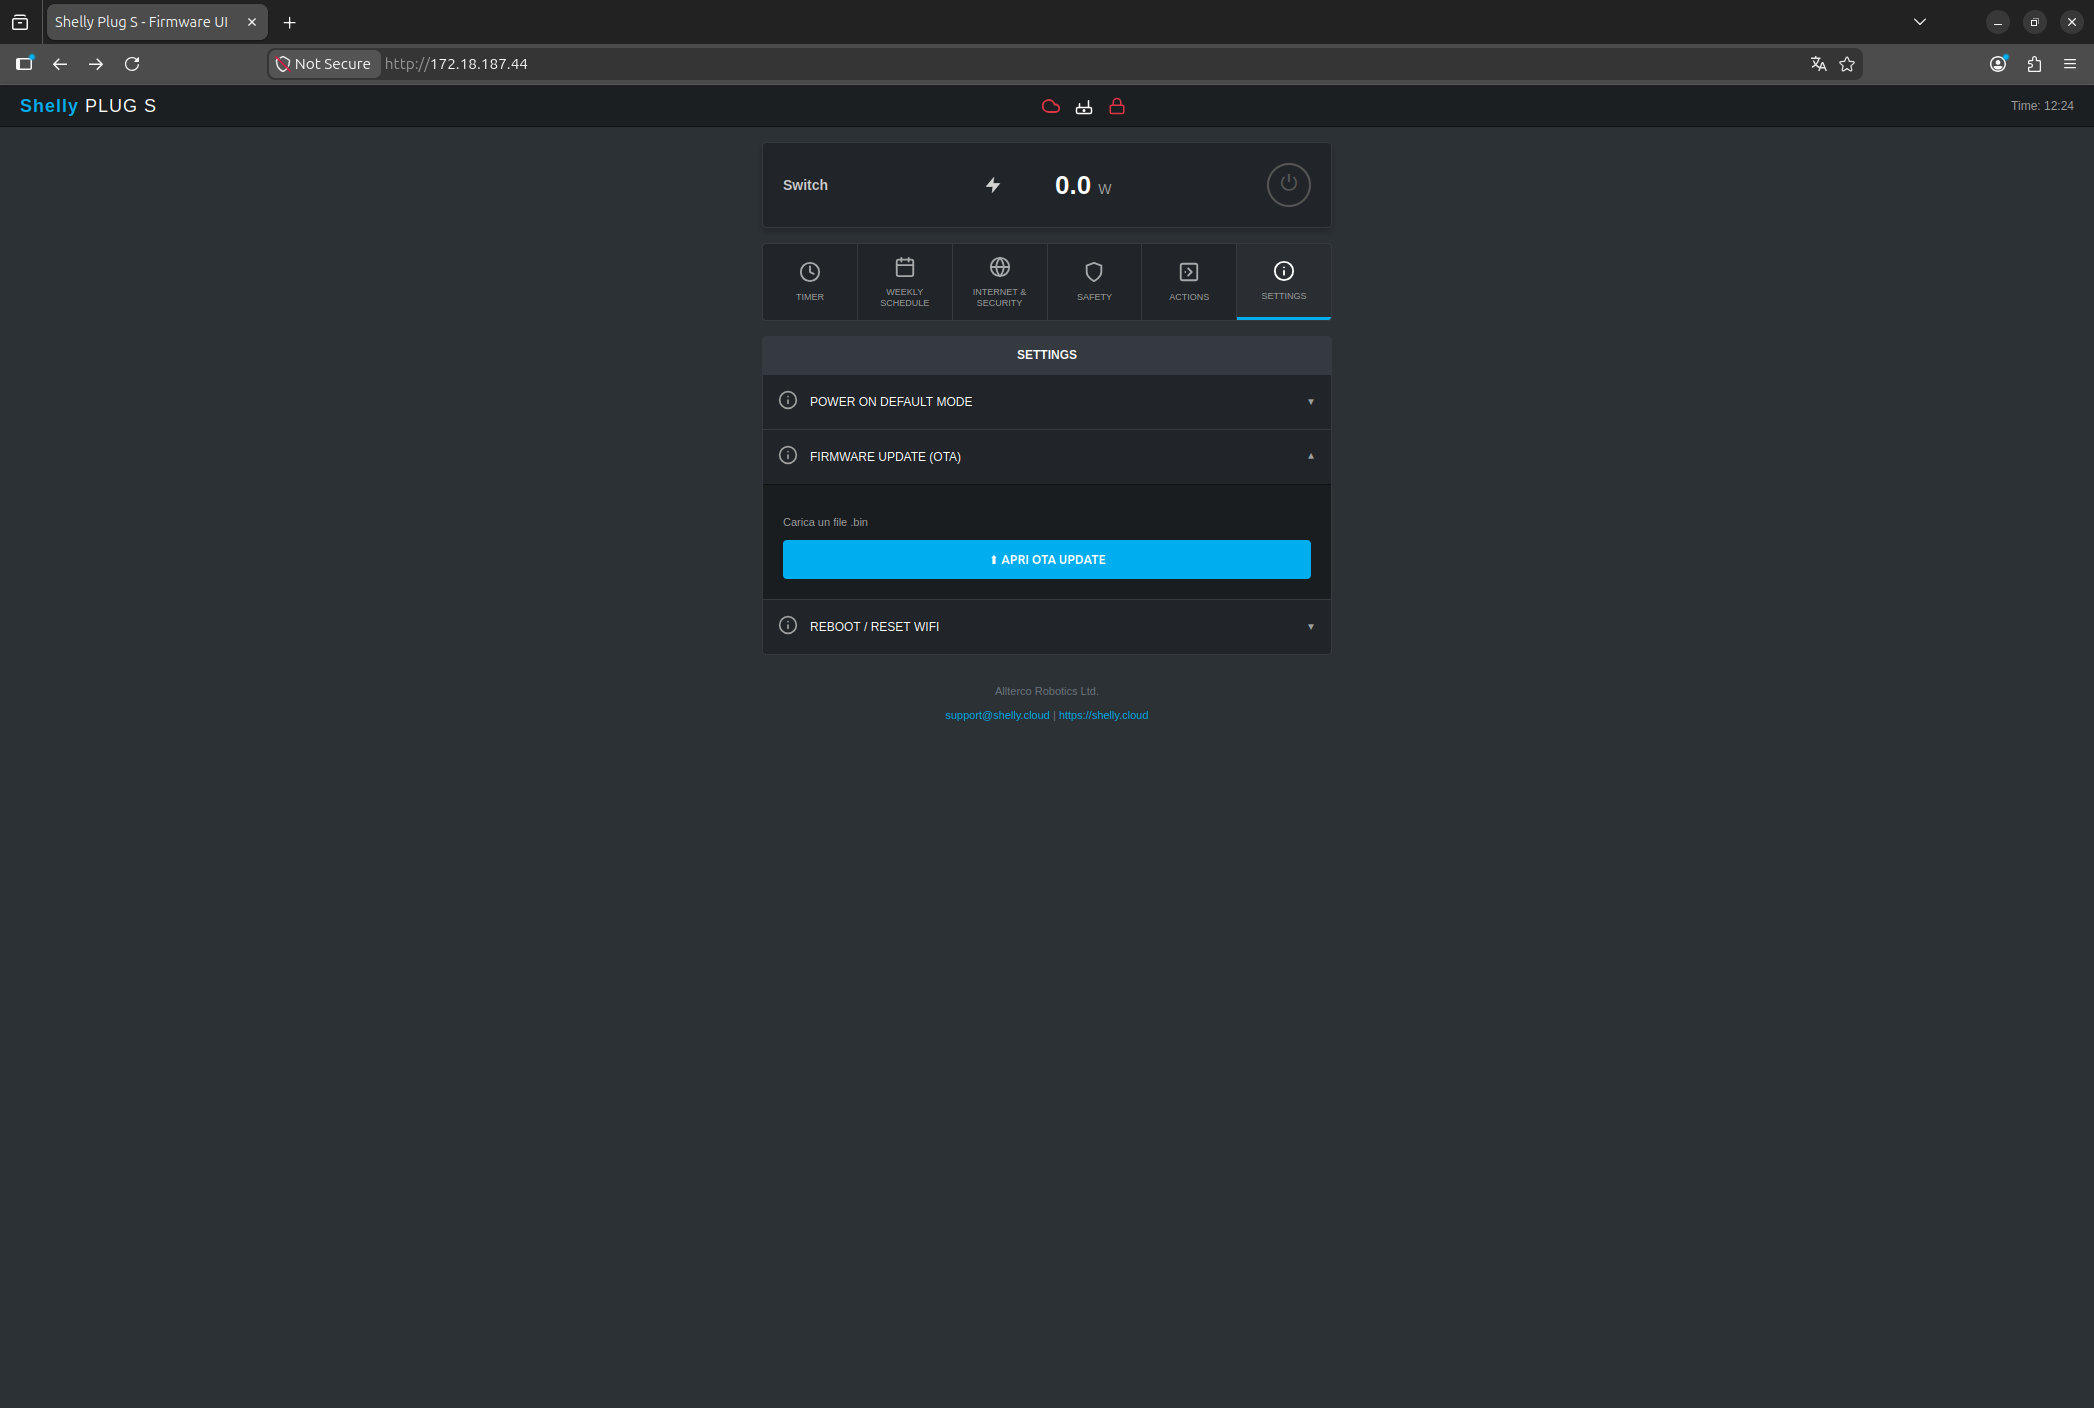
\includegraphics[width=0.90\linewidth]{Images/Fase3/OtaProtetto0.png}
    \caption{Settings page of the hardened firmware showing the ``Firmware Update (OTA)'' option}
    \label{fig:ota_settings}
\end{figure}

\begin{figure}[H]
    \centering
    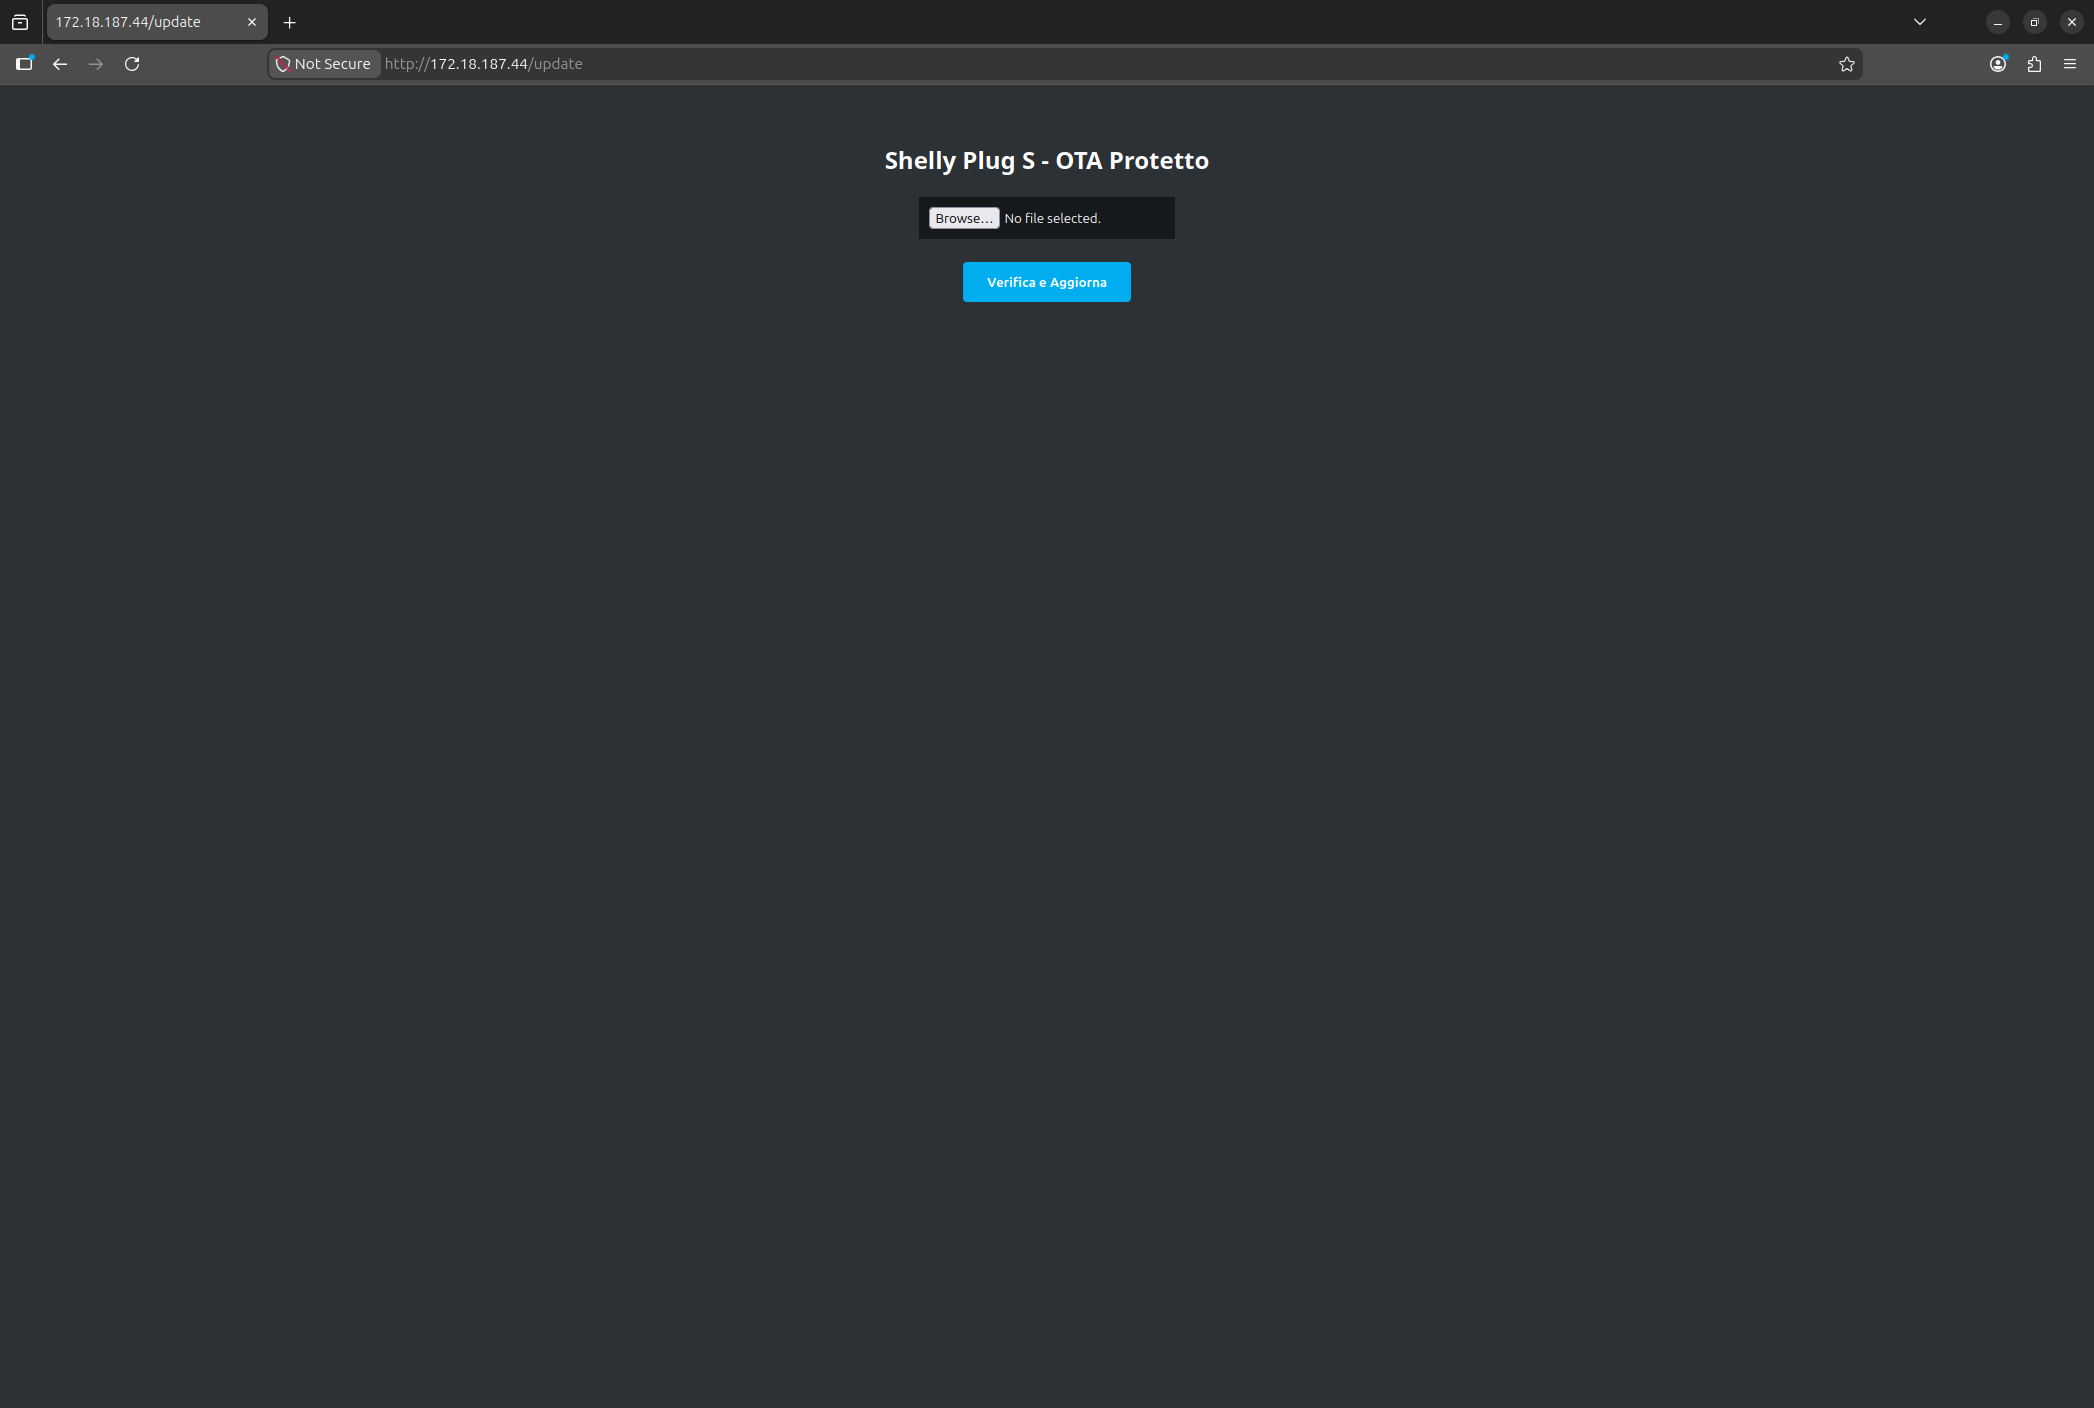
\includegraphics[width=0.90\linewidth]{Images/Fase3/OtaProtetto1.png}
    \caption{Secure OTA update page (\texttt{/update}): the user selects a signed \texttt{.bin} file for upload}
    \label{fig:ota_page}
\end{figure}

\begin{figure}[H]
    \centering
    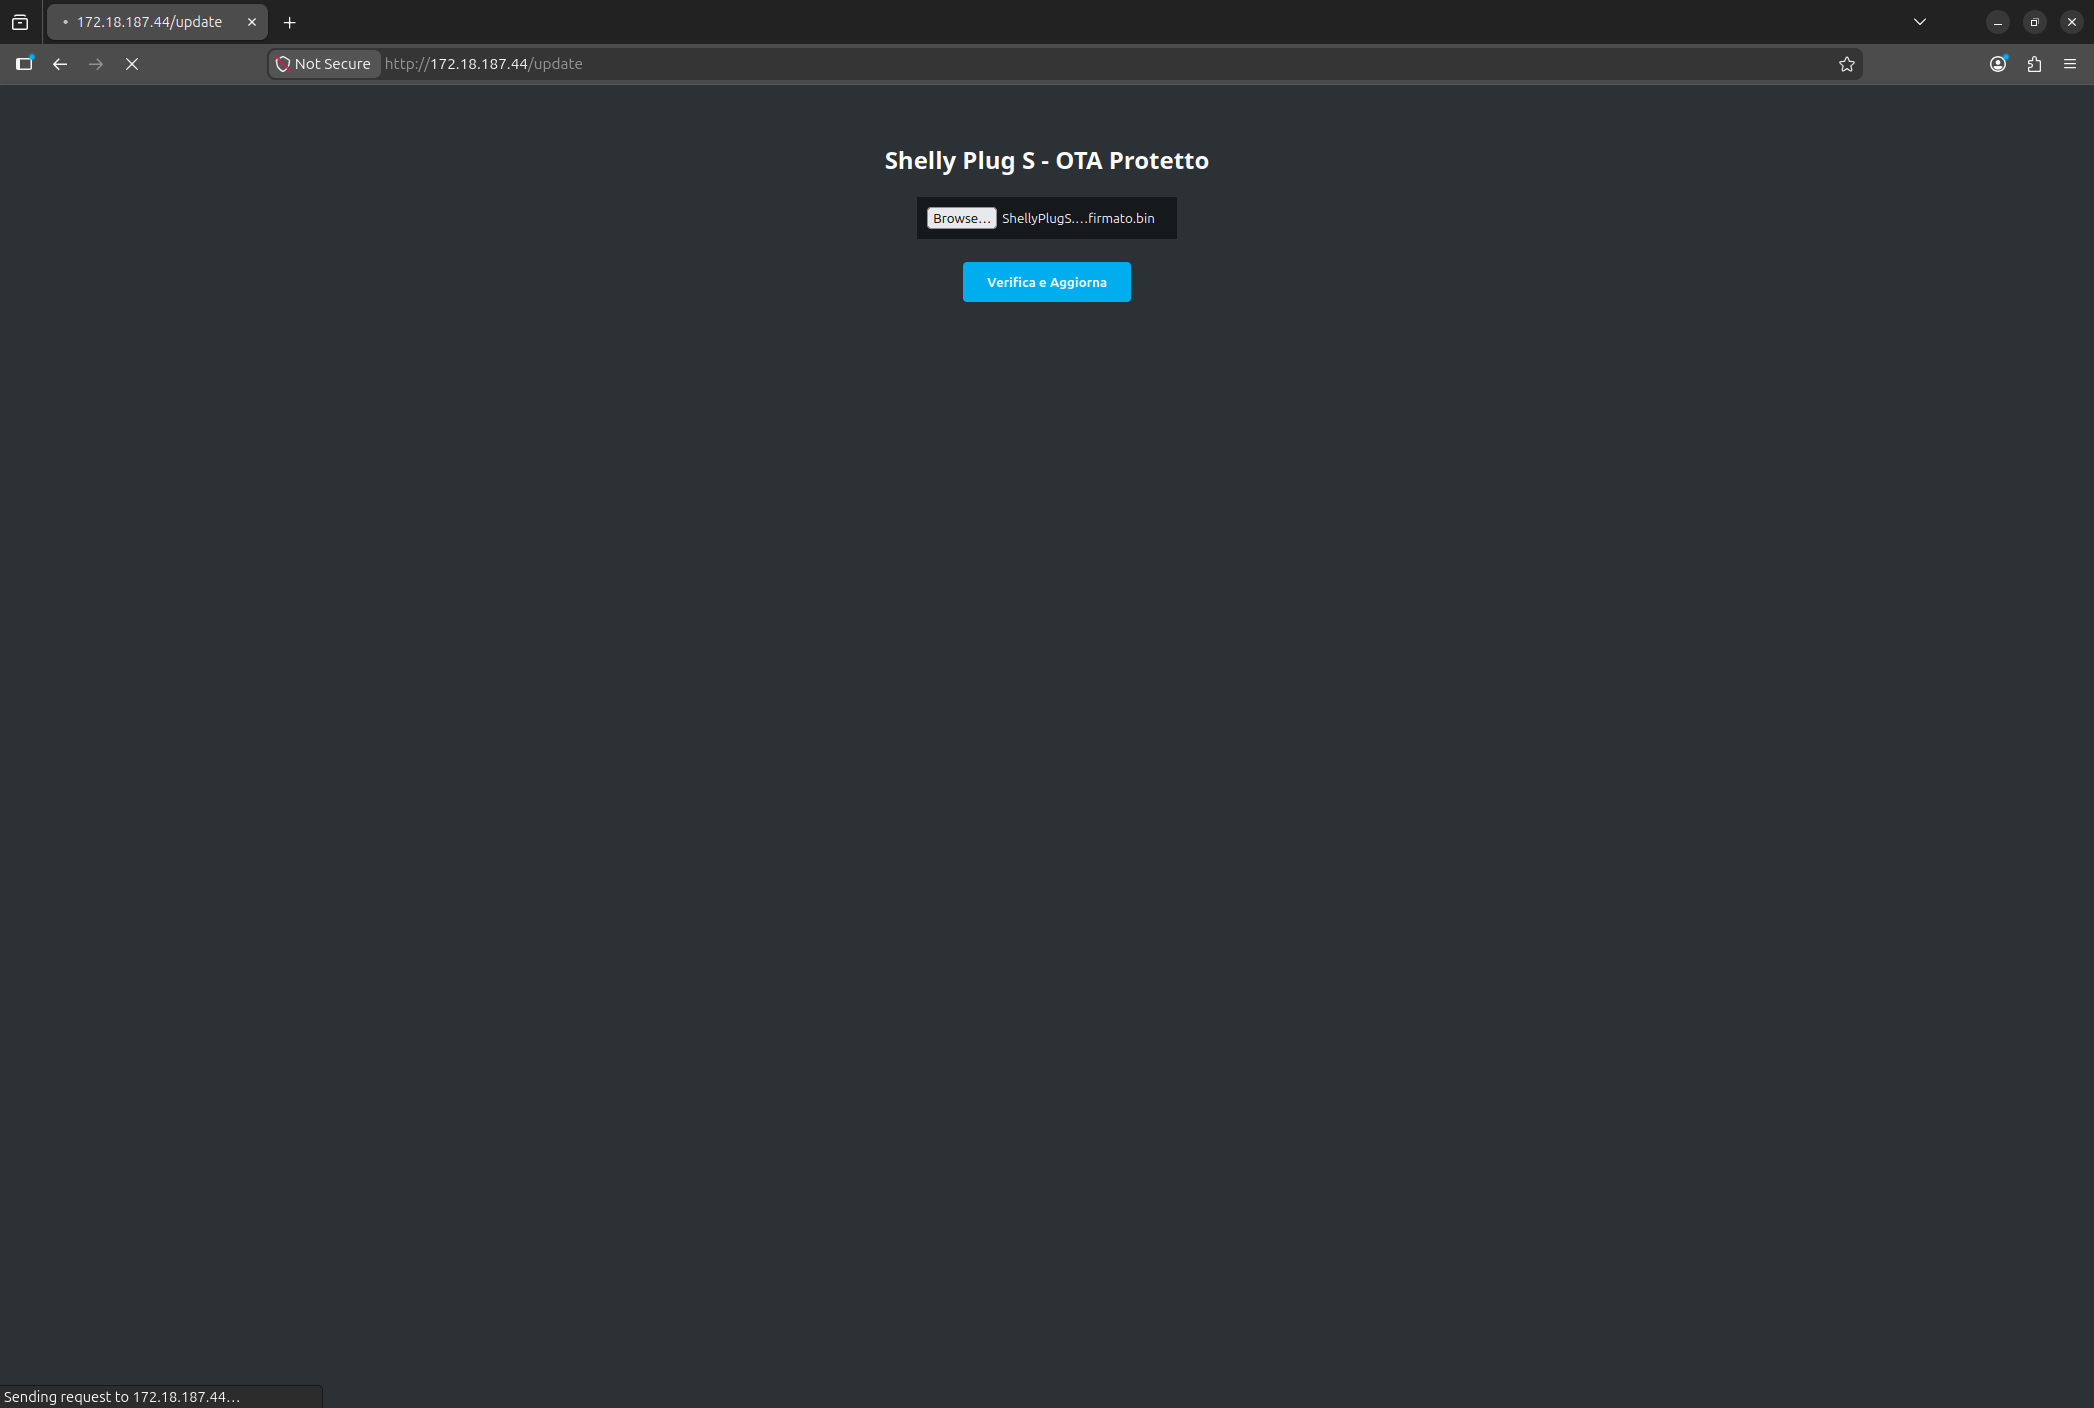
\includegraphics[width=0.90\linewidth]{Images/Fase3/OtaProtetto2.png}
    \caption{Upload in progress: the signed firmware (\texttt{ShellyPlugS...firmato.bin}) is being transmitted to the device}
    \label{fig:ota_uploading}
\end{figure}

\begin{figure}[H]
    \centering
    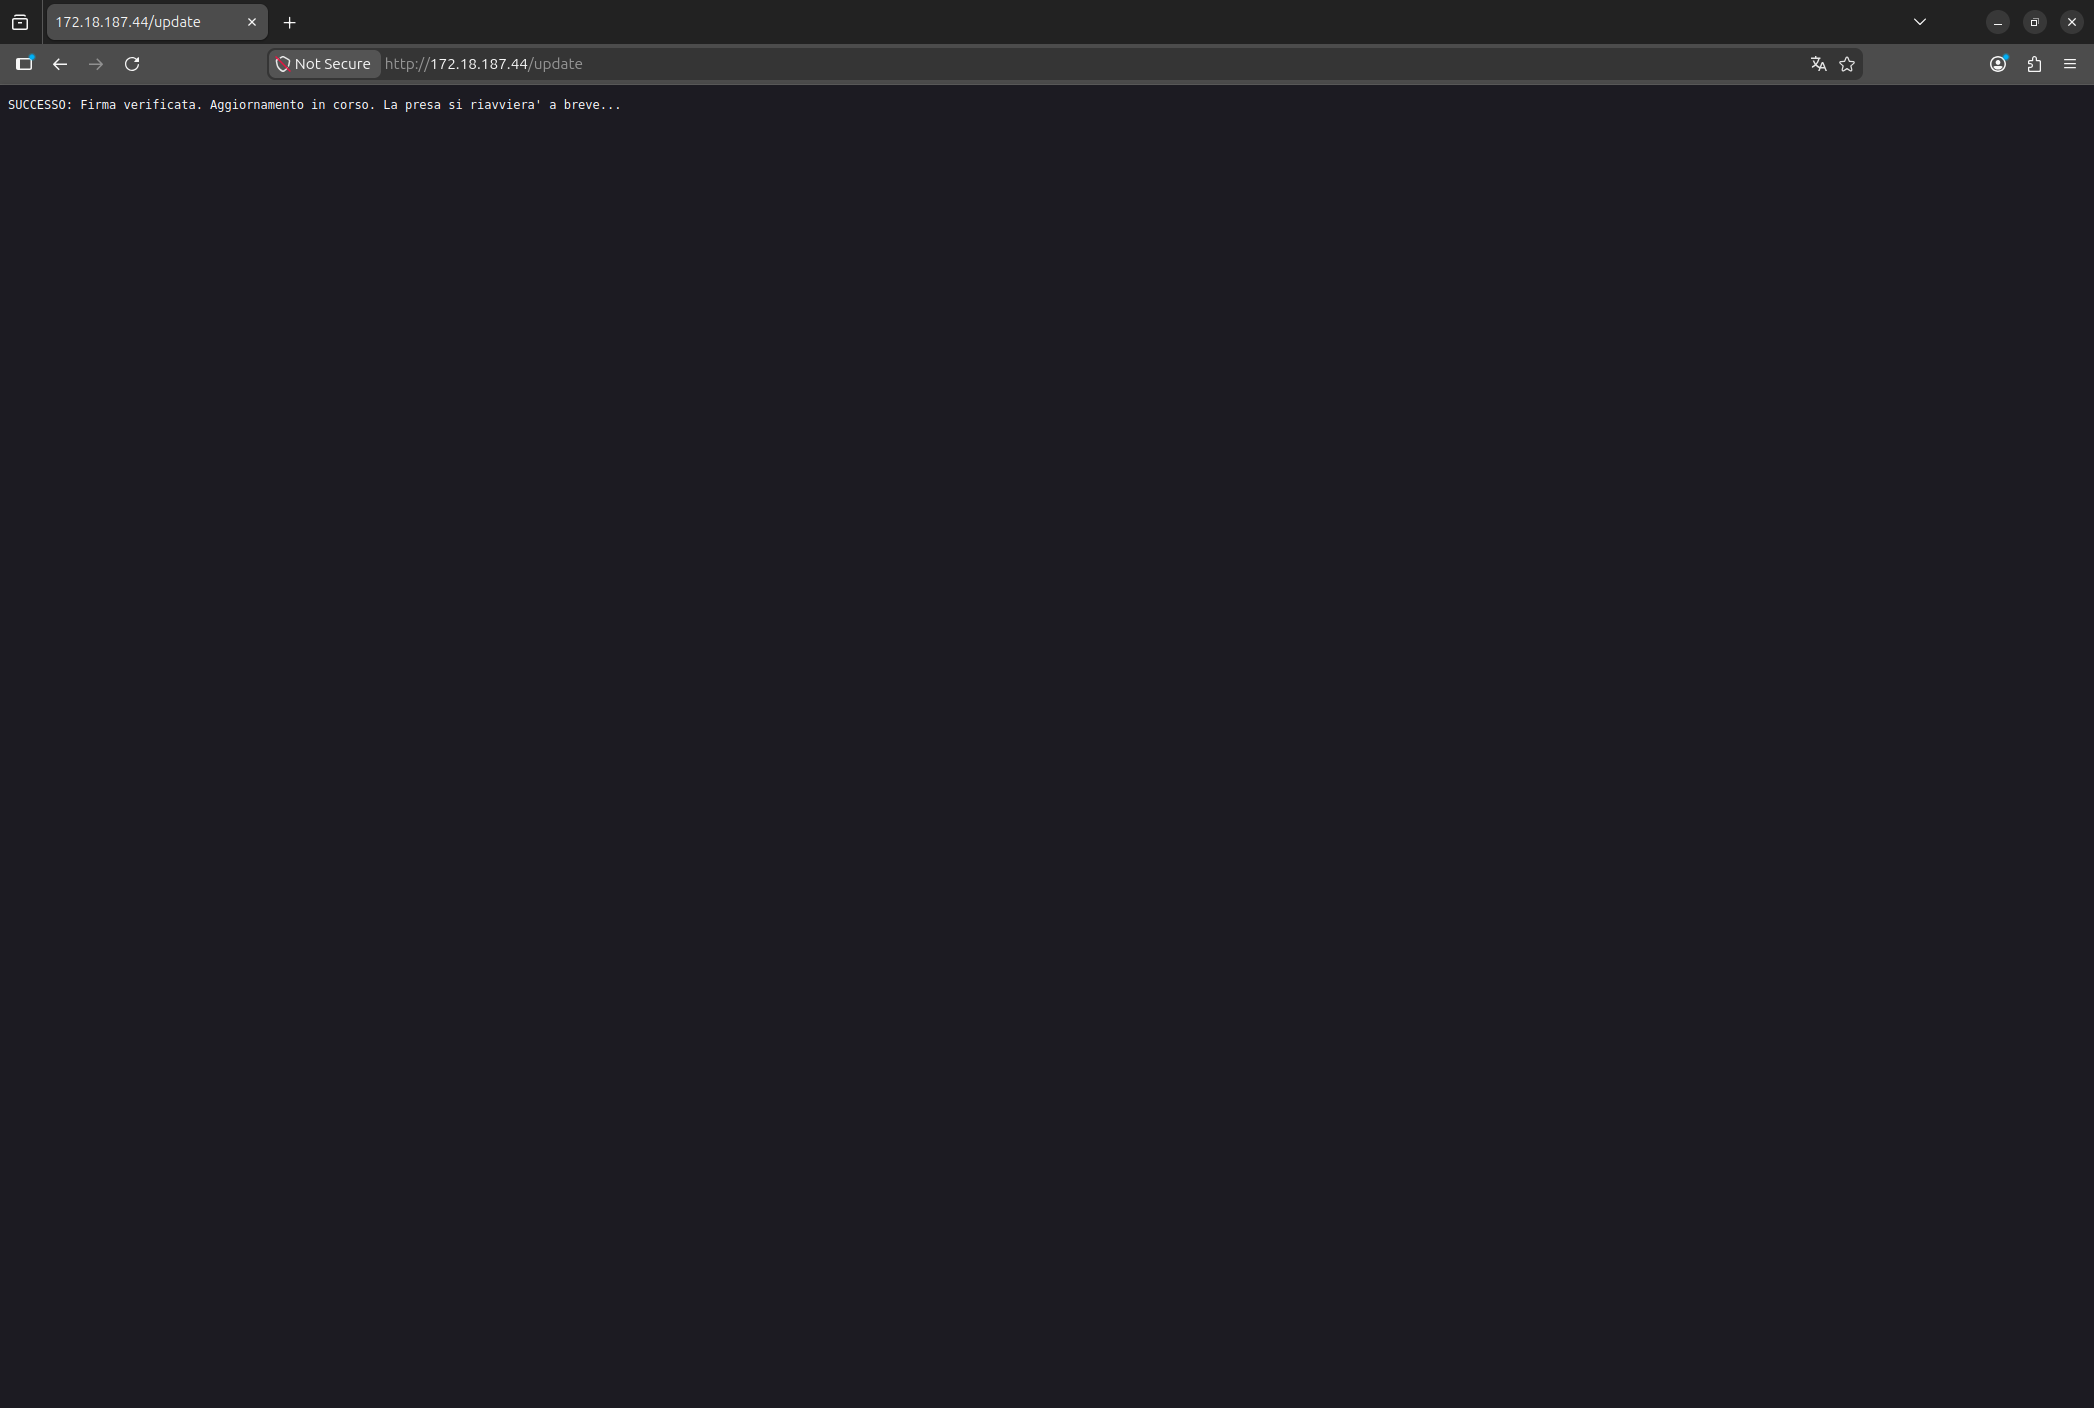
\includegraphics[width=0.90\linewidth]{Images/Fase3/OtaProtetto3.png}
    \caption{Successful verification: the device confirms ``SUCCESSO: Firma verificata. Aggiornamento in corso. La presa si riavviera' a breve...''}
    \label{fig:ota_success}
\end{figure}


\subsubsection{Demonstration: Rejected Unsigned Firmware}

To validate the rejection mechanism, an unsigned firmware binary (the raw \texttt{ShellyPlugS\_3.ino.bin} without the appended signature) was uploaded to the device. Figures~\ref{fig:ota_error1}--\ref{fig:ota_error2} show the result:

\begin{figure}[H]
    \centering
    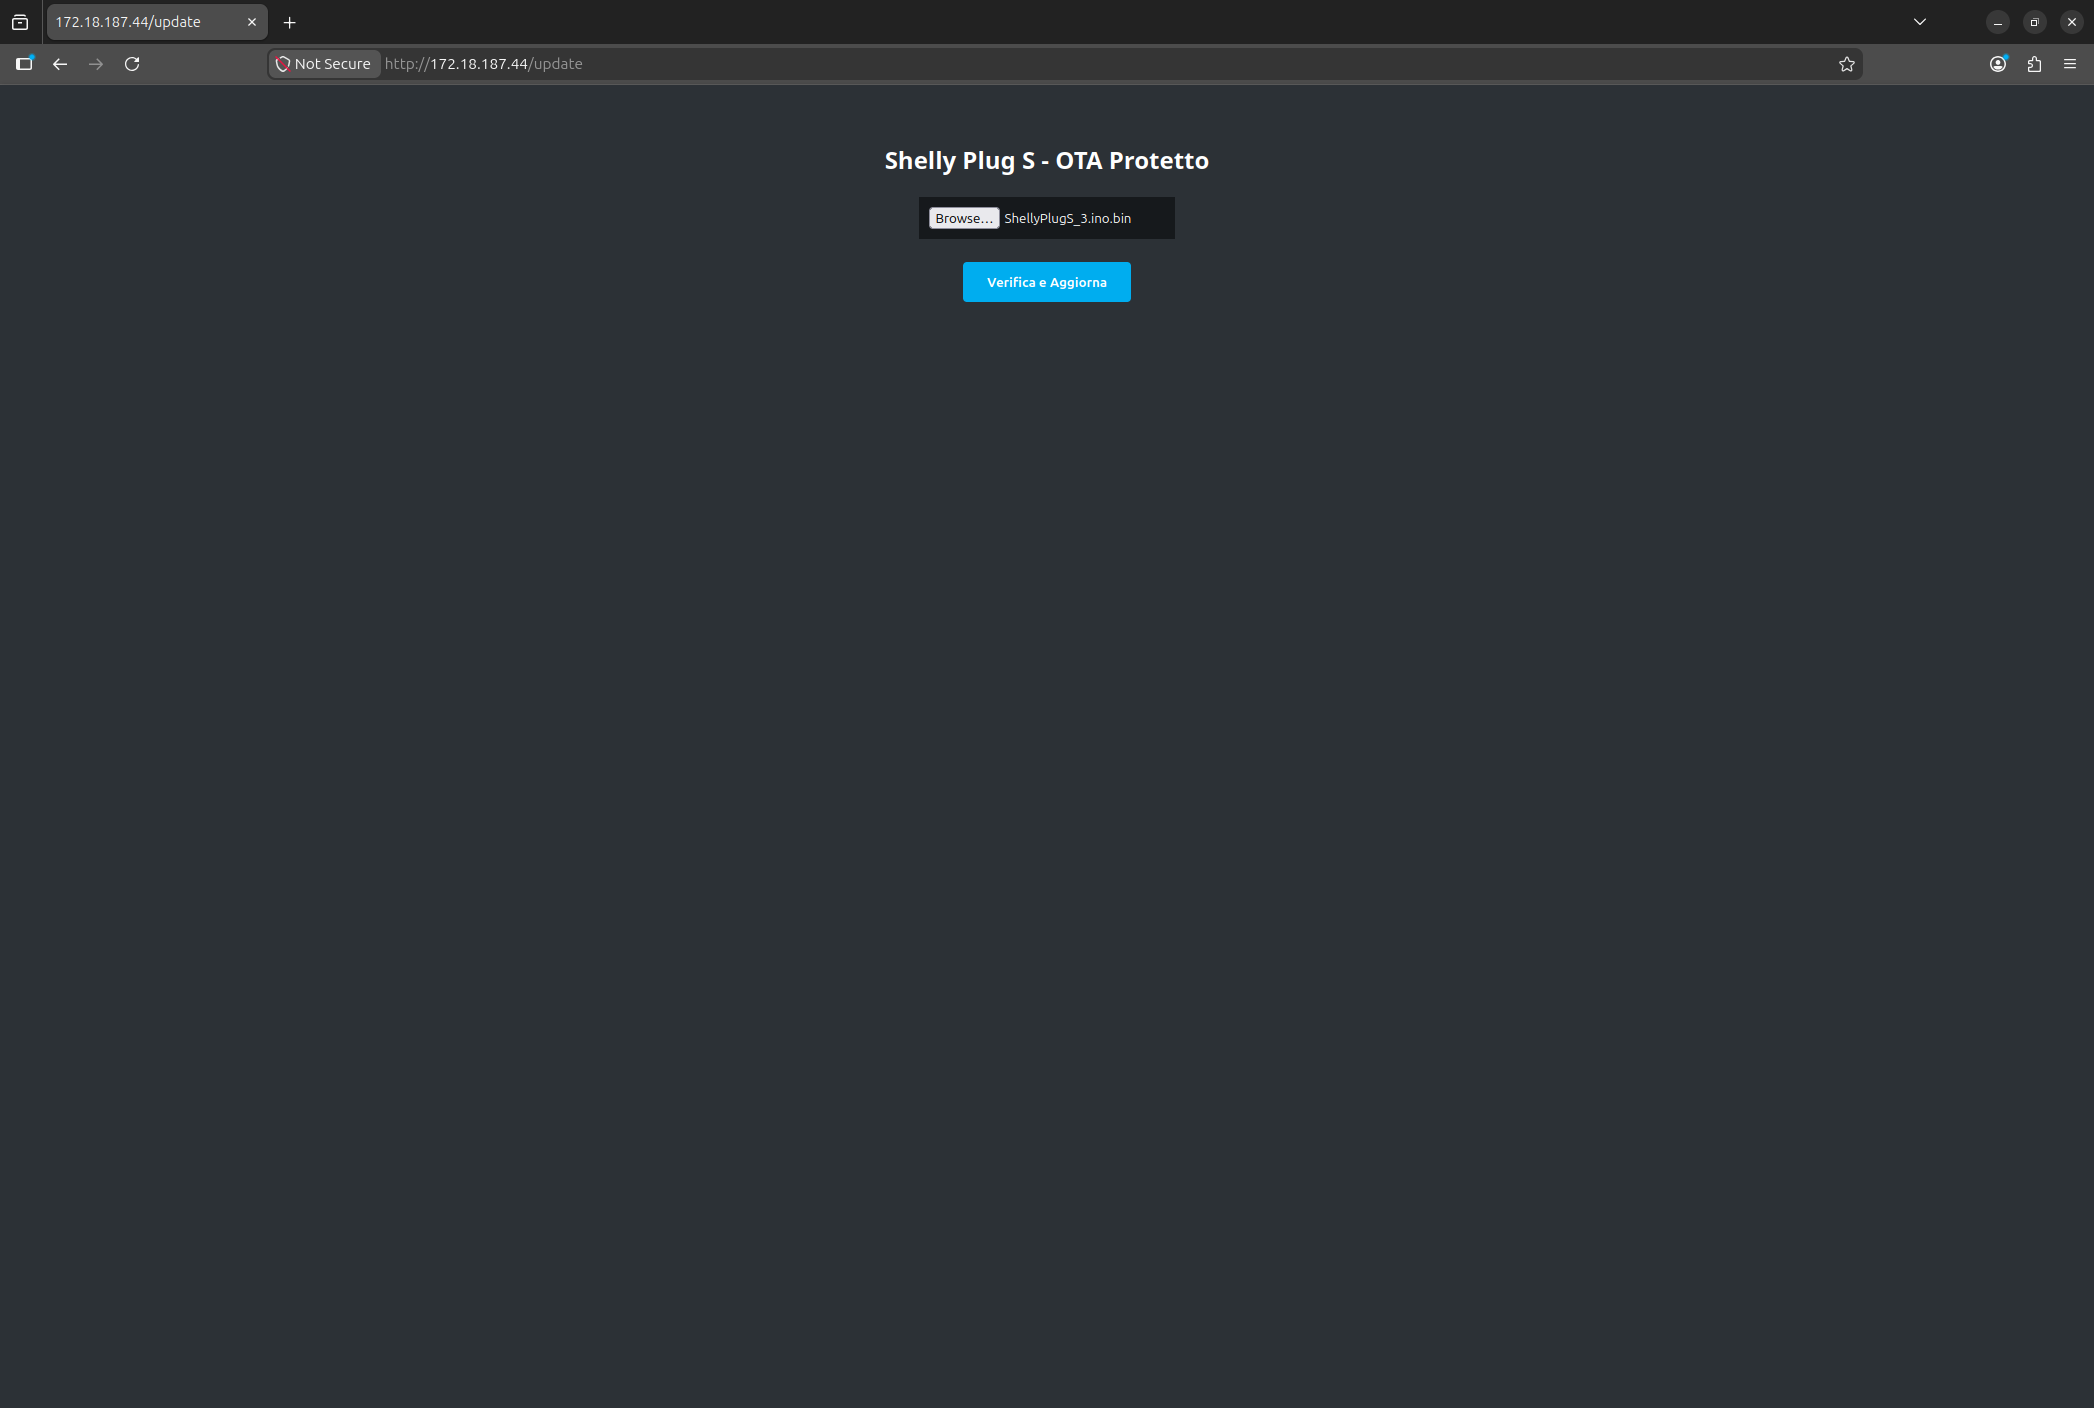
\includegraphics[width=0.90\linewidth]{Images/Fase3/OTAProtettoErrore1.png}
    \caption{Upload of an unsigned binary (\texttt{ShellyPlugS\_3.ino.bin}) — the file lacks the RSA signature trailer}
    \label{fig:ota_error1}
\end{figure}

\begin{figure}[H]
    \centering
    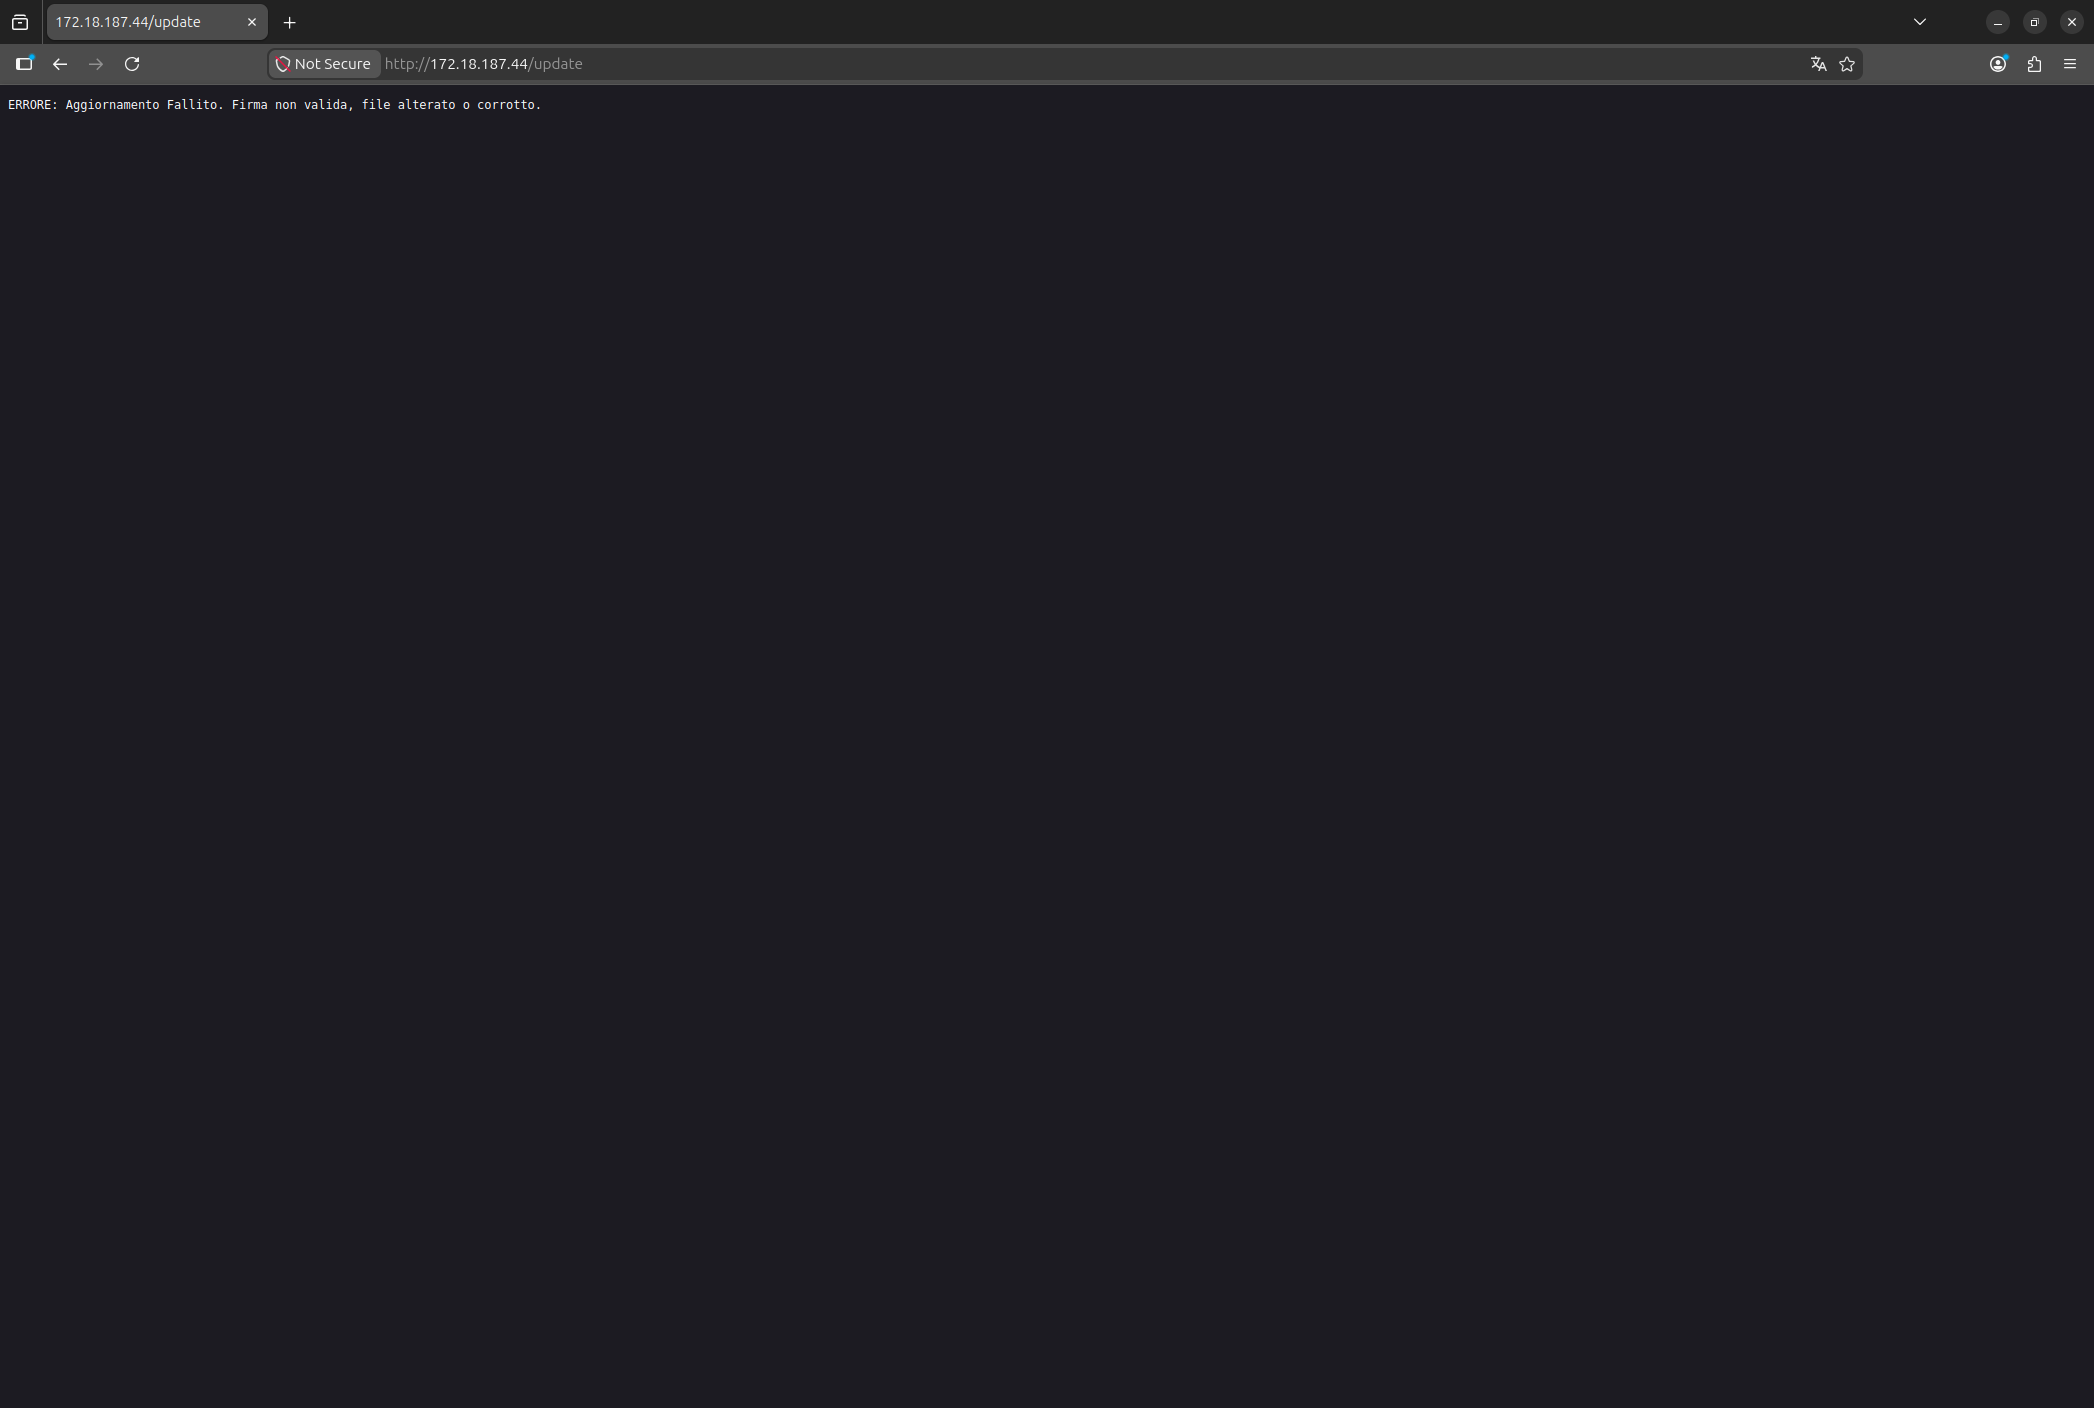
\includegraphics[width=0.90\linewidth]{Images/Fase3/OtaProtettoErrore2.png}
    \caption{Rejection: the device responds with ``ERRORE: Aggiornamento Fallito. Firma non valida, file alterato o corrotto.'', confirming the signature verification rejected the unsigned binary}
    \label{fig:ota_error2}
\end{figure}

\noindent The device correctly identifies that the uploaded binary does not carry a valid signature and refuses to apply the update. The existing firmware remains intact, and the device continues to operate normally.


\section{Ensuring Confidentiality and Authenticity}
\label{sec:confidentiality}

The second major vulnerability exploited in Phase~1 was the use of \textbf{unencrypted MQTT} (port 1883), which allowed any network observer to intercept telemetry data (power, energy, temperature) and control commands (relay on/off) in plaintext. This section describes the migration to MQTTS and the implementation of mutual TLS authentication to address both confidentiality and authenticity.


\subsection{Secure MQTT (MQTTS)}

The hardened firmware replaces the standard \texttt{WiFiClient} used in Phase~2 with a \texttt{BearSSL::WiFiClientSecure} instance (Figure~\ref{fig:mqtts0}), which wraps all TCP communication in a TLS 1.2 encrypted tunnel. The MQTT client (\texttt{PubSubClient}) is then instantiated on top of this secure transport, transparently encrypting all MQTT traffic.

\begin{figure}[H]
    \centering
    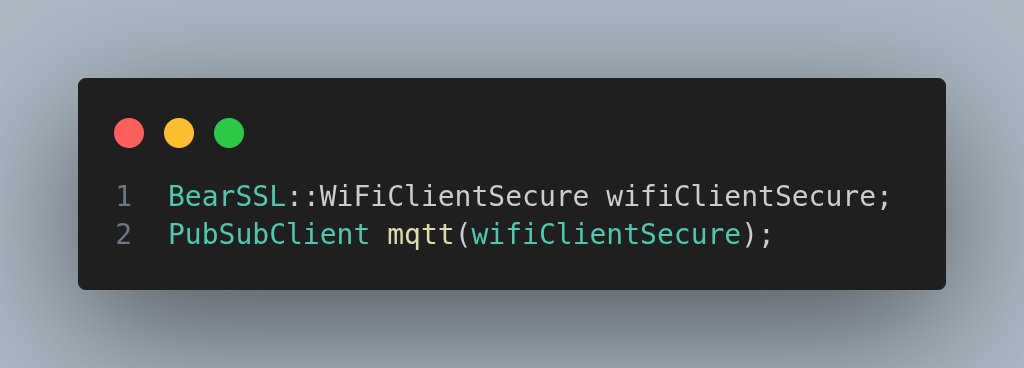
\includegraphics[width=0.55\linewidth]{Images/Fase3/mqtts0.png}
    \caption{Secure client declaration: \texttt{BearSSL::WiFiClientSecure} replaces the plaintext \texttt{WiFiClient}, and the \texttt{PubSubClient} is wrapped around it}
    \label{fig:mqtts0}
\end{figure}

\noindent The MQTT connection is configured to use \textbf{port 8883} (the standard MQTTS port) instead of the plaintext port 1883:

\begin{verbatim}
char mqtt_port[6] = "8883";
\end{verbatim}

\subsubsection{NTP Synchronization}

TLS certificate validation requires an accurate system clock to verify certificate validity periods (the \texttt{notBefore} and \texttt{notAfter} fields in X.509 certificates). Since the ESP8266 does not have a Real-Time Clock (RTC) and loses its time reference on every power cycle, the firmware implements NTP (Network Time Protocol) synchronization at startup (Figure~\ref{fig:mqtts1}). The \texttt{syncNTP()} function queries \texttt{pool.ntp.org} and \texttt{time.nist.gov} with a 10-second timeout. If synchronization fails, the firmware logs a warning indicating that TLS may not function correctly.

\subsubsection{TLS Configuration}

The \texttt{setupTLS()} function (Figure~\ref{fig:mqtts1}) configures the BearSSL client for mutual TLS authentication by loading three cryptographic objects:

\begin{enumerate}
    \item \textbf{CA Certificate} (\texttt{ca\_cert}): The Certificate Authority certificate used to verify the broker's identity. Set via \texttt{setTrustAnchors()}.
    \item \textbf{Client Certificate} (\texttt{client\_cert}): The device's X.509 certificate, presented to the broker during the TLS handshake. Set via \texttt{setClientECCert()}.
    \item \textbf{Client Private Key} (\texttt{client\_key}): The ECC private key corresponding to the client certificate, used to prove ownership. Set via \texttt{setClientECCert()}.
\end{enumerate}

\begin{figure}[H]
    \centering
    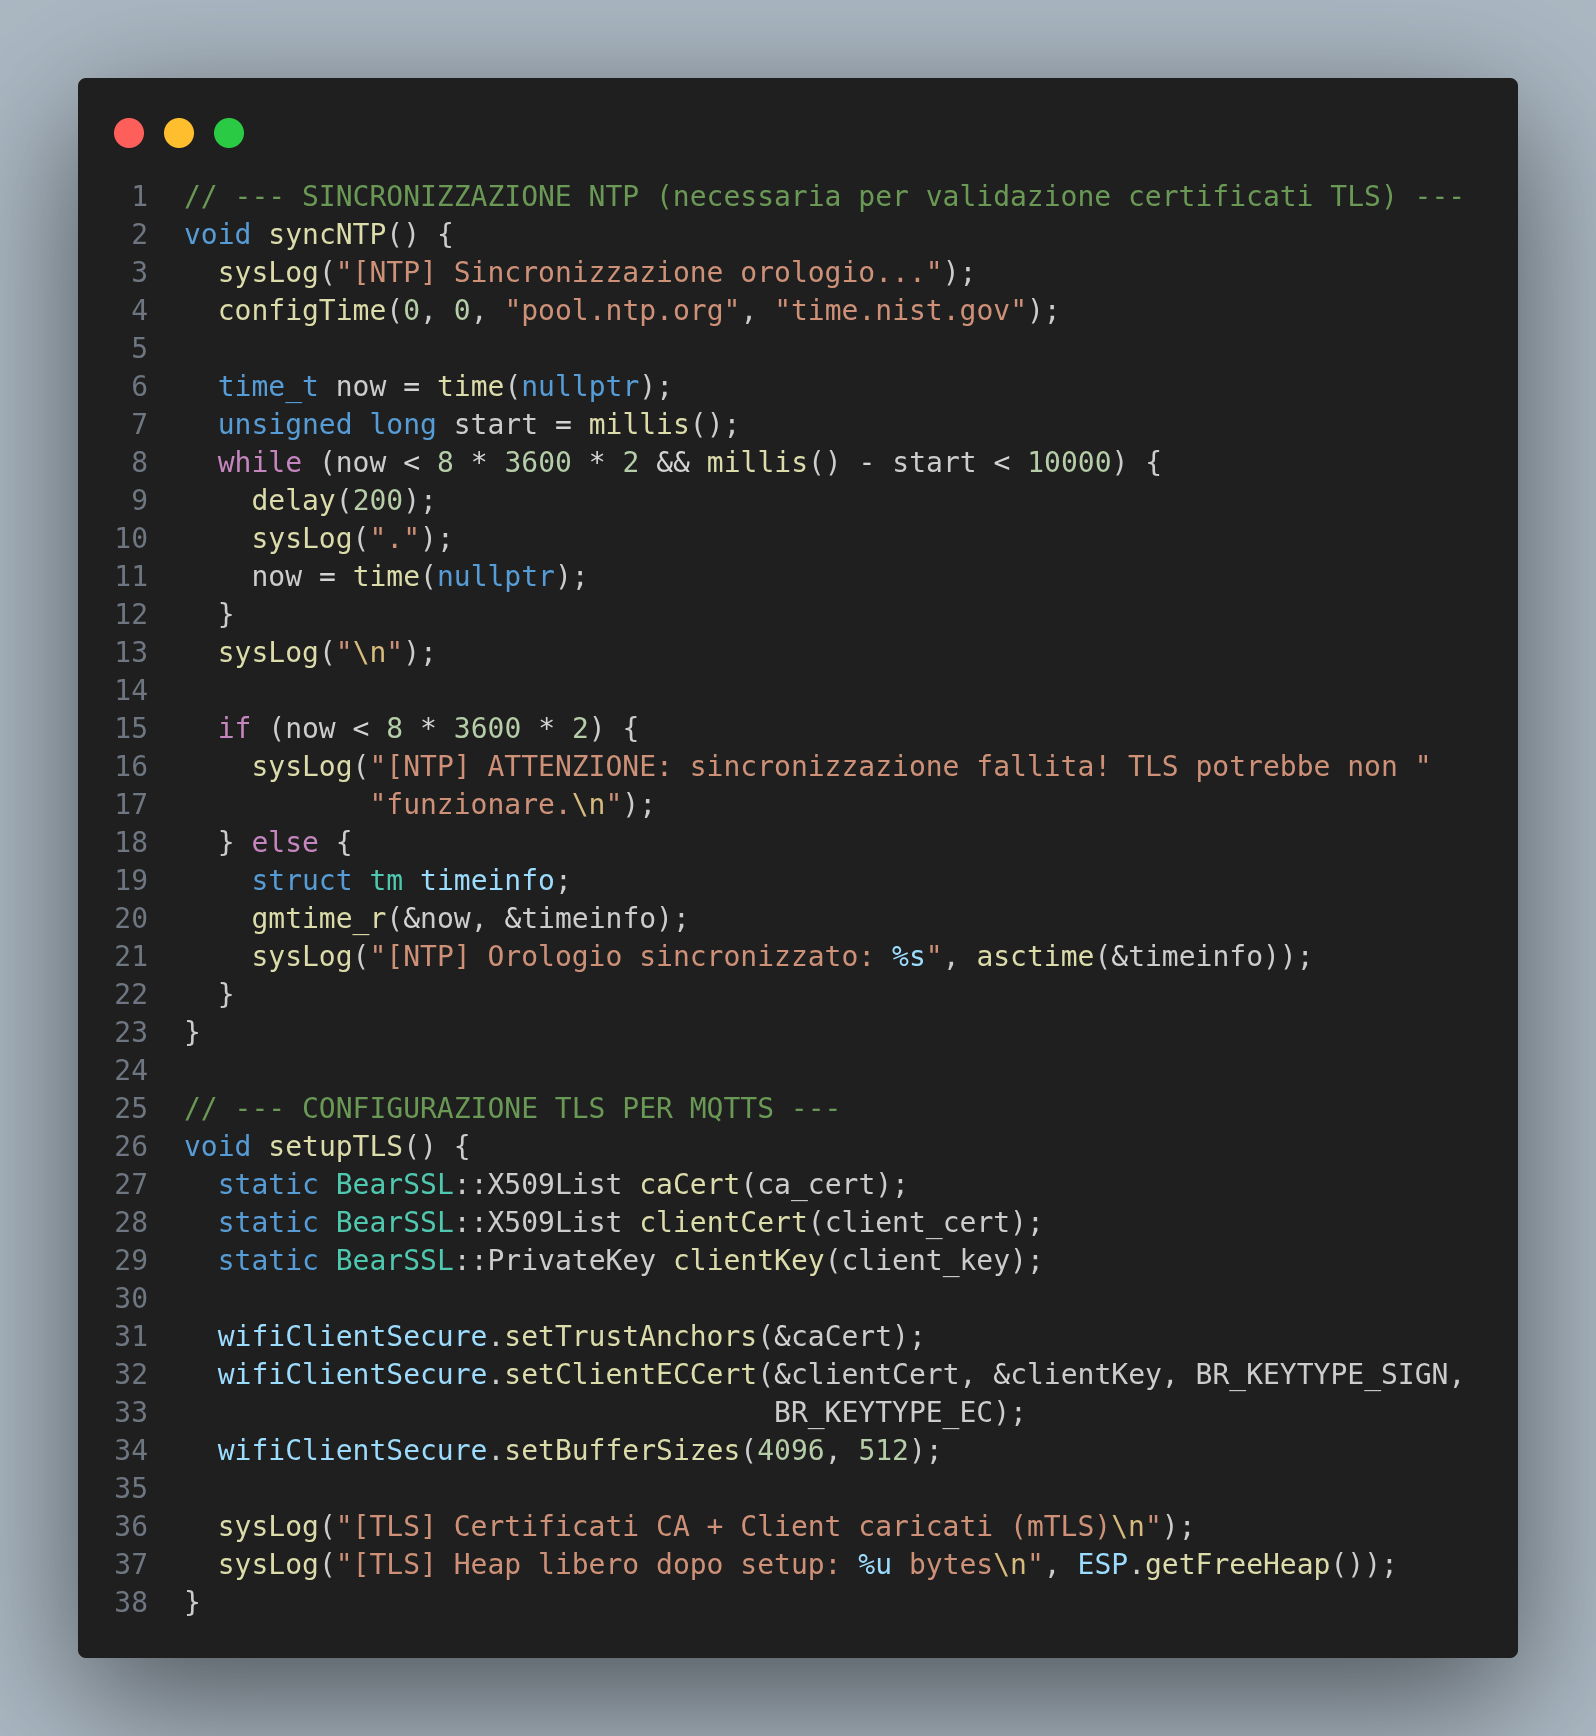
\includegraphics[width=0.80\linewidth]{Images/Fase3/mqtts1.png}
    \caption{NTP synchronization and TLS configuration: the firmware synchronizes the system clock and loads CA, client certificate, and client private key for mTLS}
    \label{fig:mqtts1}
\end{figure}

\noindent The TLS buffer sizes are explicitly configured to accommodate the ESP8266's limited memory:

\begin{verbatim}
wifiClientSecure.setBufferSizes(4096, 512);
\end{verbatim}

\noindent This sets a 4096-byte receive buffer and a 512-byte send buffer, representing a careful trade-off between TLS functionality and the approximately 50\,KB of heap available on the ESP8266.

\subsubsection{Mitigation Effectiveness}

This countermeasure directly addresses the \textbf{Information Disclosure} threat identified in Phase~1:

\begin{itemize}
    \item \textbf{Before (Phase~1/2)}: All MQTT traffic was transmitted in plaintext on port 1883. Any attacker on the local network could use Wireshark to intercept power, energy, temperature, and relay state data.
    
    \item \textbf{After (Phase~3)}: All MQTT traffic is encrypted using TLS 1.2 on port 8883. Even if an attacker captures the packets, the payload is encrypted and appears as opaque ``Application Data'' in Wireshark.
\end{itemize}


\subsection{Mutual Authentication (mTLS)}

While standard TLS ensures confidentiality by encrypting the communication channel, it only authenticates the \emph{server} (broker) to the \emph{client} (device). Mutual TLS (mTLS) extends this by also requiring the client to present a valid certificate to the server, ensuring \textbf{bidirectional authentication}. This prevents unauthorized devices from connecting to the MQTT broker and unauthorized brokers from impersonating the legitimate server.

\subsubsection{Certificate Hierarchy and Generation}

The mTLS infrastructure is built on a \textbf{private Certificate Authority (CA)} using Elliptic Curve Cryptography (ECC) with the \texttt{prime256v1} (P-256) curve. ECC was chosen over RSA for the TLS certificates because it provides equivalent security with significantly smaller key sizes (256-bit ECC $\approx$ 3072-bit RSA), which is critical for the memory-constrained ESP8266.

\medskip
\noindent The PKI hierarchy consists of four entities, each with its own certificate directory on the server (Figure~\ref{fig:certificati}):

\begin{figure}[H]
    \centering
    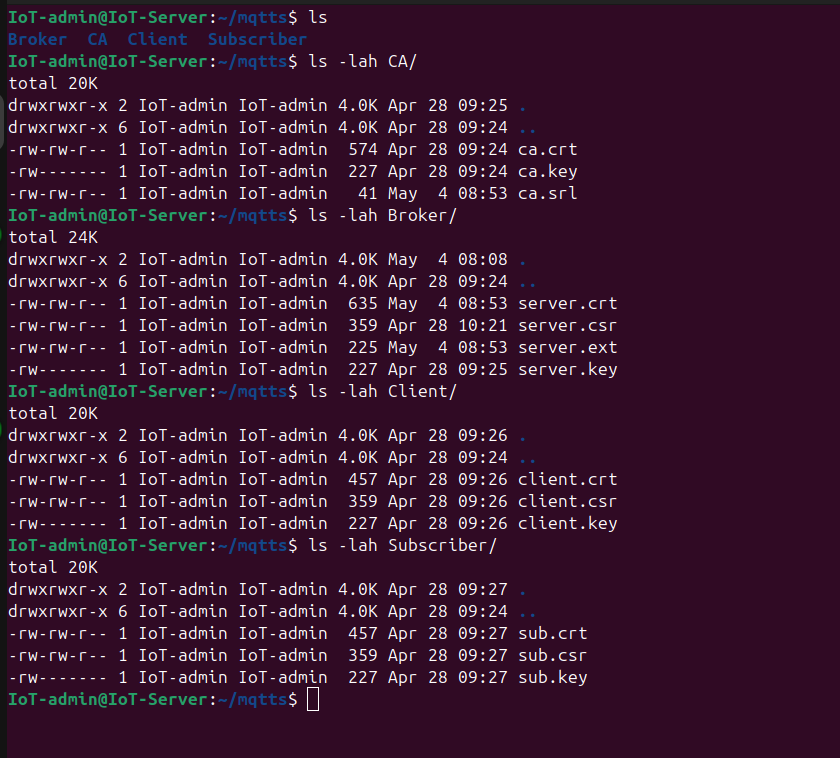
\includegraphics[width=0.75\linewidth]{Images/Fase3/Certificati.png}
    \caption{Certificate directory structure: separate directories for CA, Broker, Client (Shelly device), and Subscriber, each containing its certificate (\texttt{.crt}), private key (\texttt{.key}), and CSR (\texttt{.csr})}
    \label{fig:certificati}
\end{figure}

\noindent The certificates were generated using the following \texttt{openssl} commands:

\medskip
\noindent \textbf{1. Certificate Authority (CA):}

The self-signed root CA certificate is generated with a validity of 10 years:

\begin{bashcode}
# Generate CA private key (ECC P-256)
openssl ecparam -genkey -name prime256v1 -out CA/ca.key

# Generate self-signed CA certificate (10 years)
openssl req -new -x509 -key CA/ca.key -out CA/ca.crt \
    -days 3650 -subj "/CN=MyHomeCA"
\end{bashcode}

\medskip
\noindent \textbf{2. Broker Certificate:}

The broker certificate is signed by the CA. An extensions file (\texttt{server.ext}) is used to specify Subject Alternative Names (SANs), which is necessary for the broker's IP-based addressing:

\begin{bashcode}
# Generate broker private key
openssl ecparam -genkey -name prime256v1 -out Broker/server.key

# Generate Certificate Signing Request (CSR)
openssl req -new -key Broker/server.key -out Broker/server.csr \
    -subj "/CN=MQTTBroker"

# Sign the CSR with the CA (with SANs for IP-based access)
openssl x509 -req -in Broker/server.csr -CA CA/ca.crt \
    -CAkey CA/ca.key -CAcreateserial -out Broker/server.crt \
    -days 3650 -extfile Broker/server.ext
\end{bashcode}

\noindent Where \texttt{server.ext} contains:
\begin{verbatim}
subjectAltName = IP:74.161.73.178
\end{verbatim}

\medskip
\noindent \textbf{3. Client Certificate (Shelly Device):}

The client certificate identifies the Shelly Plug S device to the broker:

\begin{bashcode}
# Generate client private key
openssl ecparam -genkey -name prime256v1 -out Client/client.key

# Generate CSR
openssl req -new -key Client/client.key -out Client/client.csr \
    -subj "/CN=ShellyPlugS"

# Sign with CA
openssl x509 -req -in Client/client.csr -CA CA/ca.crt \
    -CAkey CA/ca.key -CAcreateserial -out Client/client.crt \
    -days 3650
\end{bashcode}

\medskip
\noindent \textbf{4. Subscriber Certificate:}

A separate certificate is generated for the subscriber client (e.g., a monitoring machine running \texttt{mosquitto\_sub}):

\begin{bashcode}
# Generate subscriber private key
openssl ecparam -genkey -name prime256v1 -out Subscriber/sub.key

# Generate CSR
openssl req -new -key Subscriber/sub.key -out Subscriber/sub.csr \
    -subj "/CN=Subscriber"

# Sign with CA
openssl x509 -req -in Subscriber/sub.csr -CA CA/ca.crt \
    -CAkey CA/ca.key -CAcreateserial -out Subscriber/sub.crt \
    -days 3650
\end{bashcode}

\noindent All four entities share the same CA trust anchor (\texttt{ca.crt}), creating a closed trust domain where only devices possessing a CA-signed certificate can participate in the MQTT communication.

\subsubsection{Mosquitto Broker Configuration}

The Mosquitto MQTT broker is configured to enforce mTLS by requiring client certificate verification. Figure~\ref{fig:mosquitto_mqtts} shows the relevant configuration directives in \texttt{mosquitto.conf}:

\begin{bashcode}
listener 8883
cafile /home/IoT-admin/mqtts/CA/ca.crt
certfile /home/IoT-admin/mqtts/Broker/server.crt
keyfile /home/IoT-admin/mqtts/Broker/server.key
require_certificate true
use_identity_as_username true
\end{bashcode}

\noindent Key configuration parameters:
\begin{itemize}
    \item \texttt{listener 8883}: The broker listens on the standard MQTTS port.
    \item \texttt{cafile}: The CA certificate used to validate both client and broker certificates.
    \item \texttt{certfile} / \texttt{keyfile}: The broker's own TLS certificate and private key.
    \item \texttt{require\_certificate true}: \textbf{This is the mTLS enforcement directive} — the broker will reject any client that does not present a valid, CA-signed certificate.
    \item \texttt{use\_identity\_as\_username true}: The Common Name (CN) field from the client certificate is used as the MQTT username, enabling certificate-based access control.
\end{itemize}

\subsubsection{Subscribing with mTLS}

To verify the correct operation of the MQTTS channel, the \texttt{mosquitto\_sub} command-line client was used with the subscriber's certificate and key. The following command connects to the broker on port 8883, presents the subscriber's certificate for mutual authentication, and subscribes to all topics:

\begin{bashcode}
mosquitto_sub -h 74.161.73.178 -p 8883 -t "#" -v \
    --cafile ca.crt --cert sub.crt --key sub.key
\end{bashcode}

\noindent The connection requires:
\begin{itemize}
    \item \texttt{--cafile ca.crt}: The CA certificate to verify the broker's identity.
    \item \texttt{--cert sub.crt}: The subscriber's own certificate, presented to the broker.
    \item \texttt{--key sub.key}: The subscriber's private key, proving ownership of the certificate.
\end{itemize}

\noindent Figures~\ref{fig:mosquitto_sub_mqtts} and \ref{fig:mosquitto_sub_mqtts2} show the MQTTS-encrypted telemetry data successfully received by the subscriber. The device publishes power, energy, temperature, relay state, and status information to the standard Shelly MQTT topic hierarchy, confirming full operational compatibility with the original Shelly ecosystem while maintaining encrypted transport.

\begin{figure}[H]
    \centering
    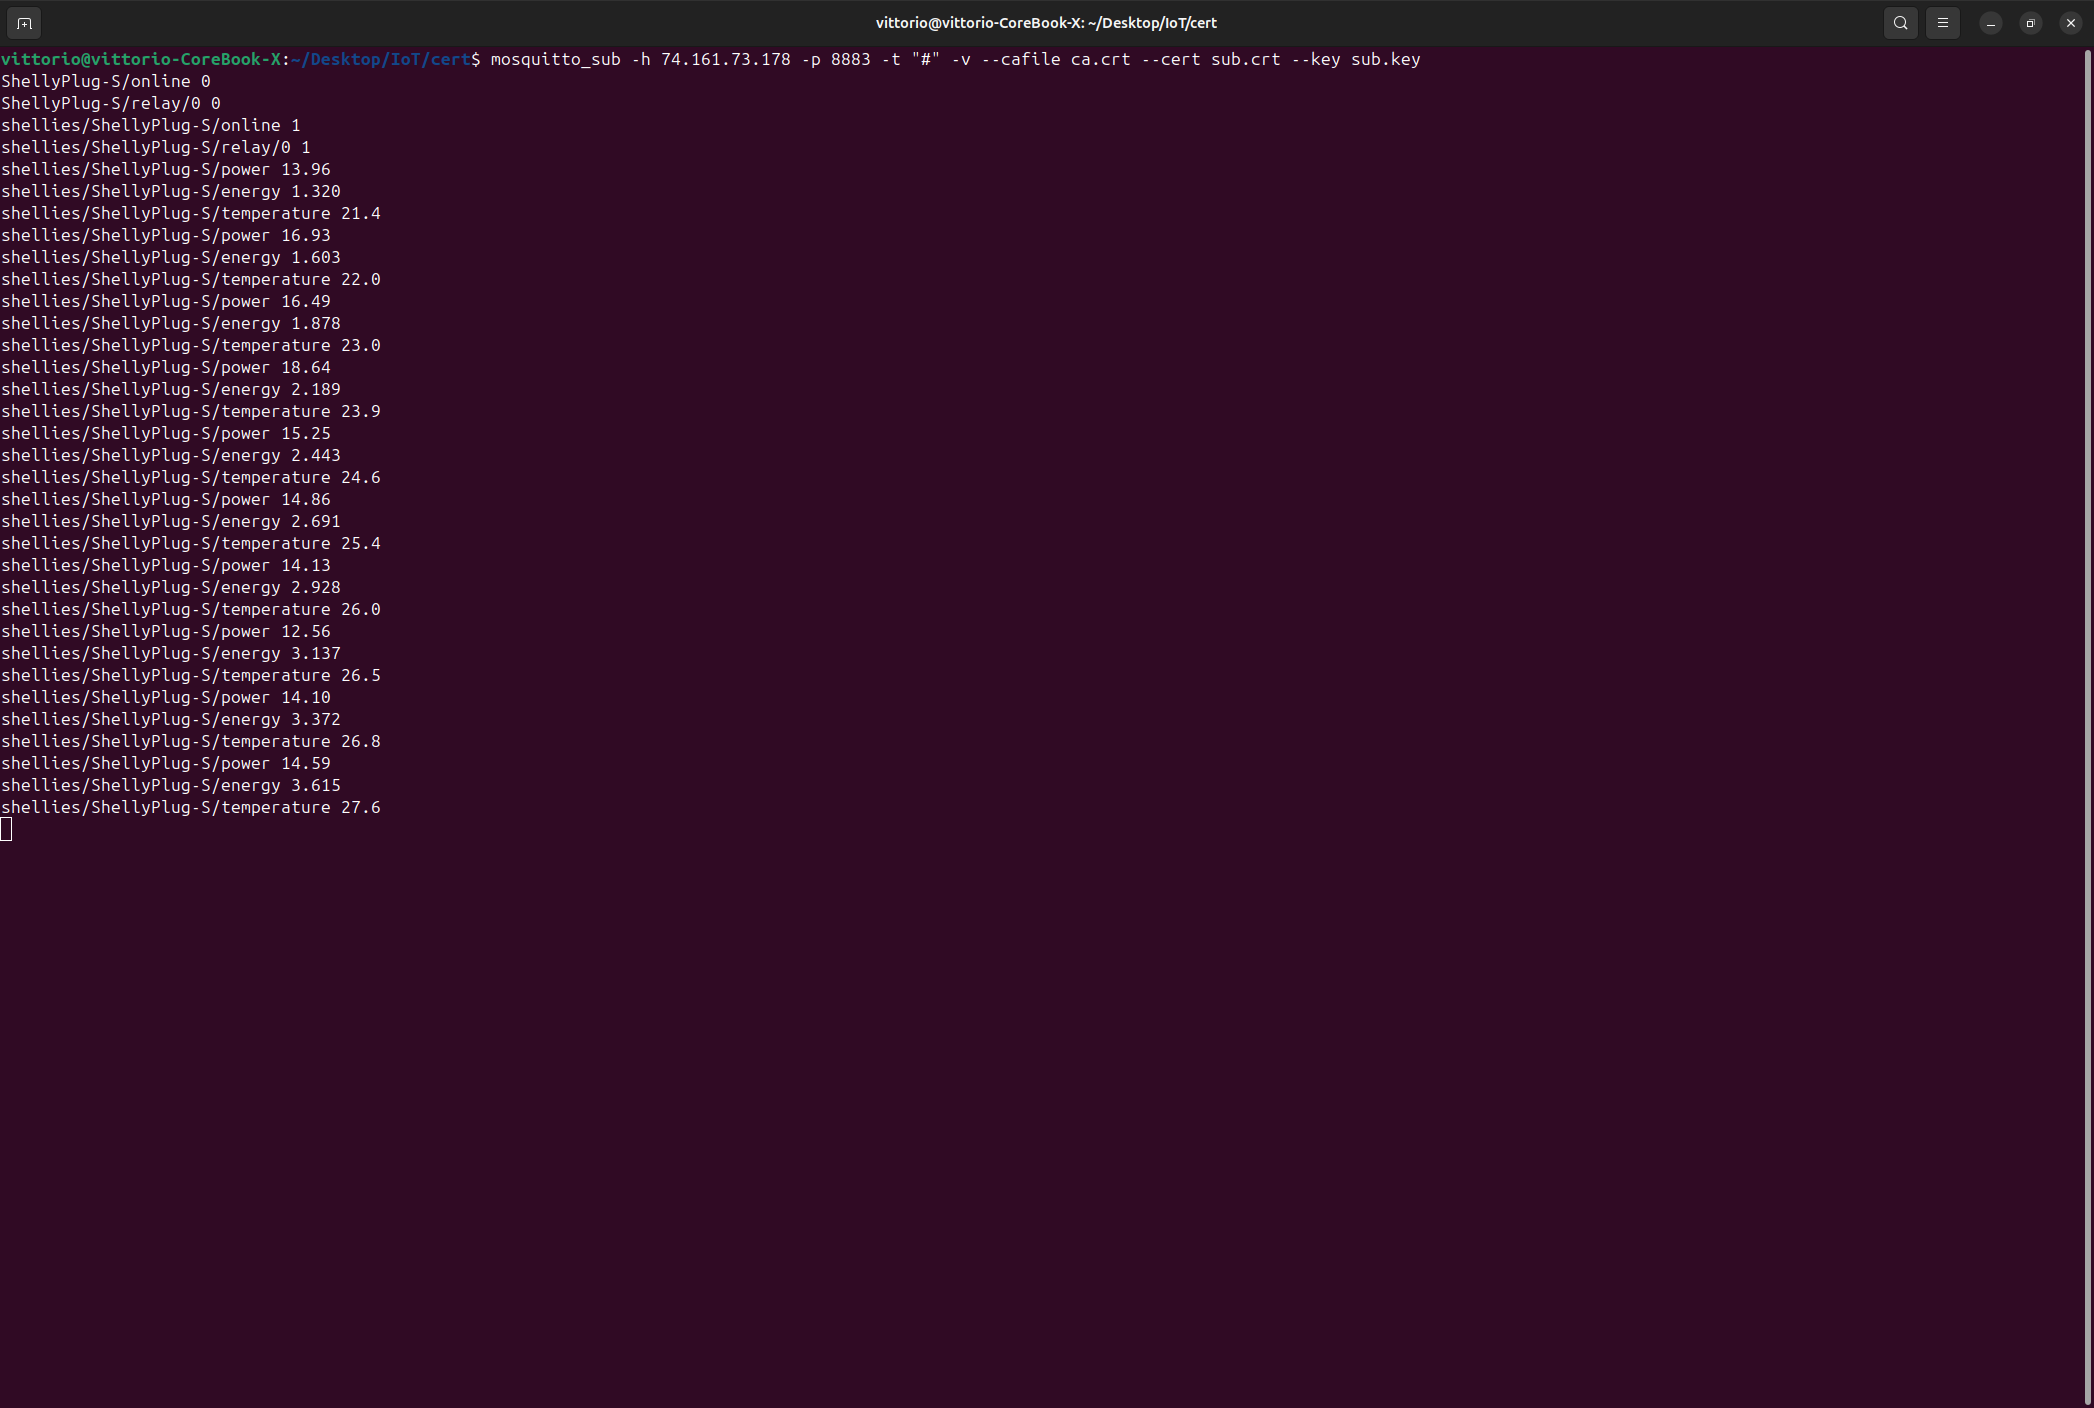
\includegraphics[width=0.95\linewidth]{Images/Fase3/MosquittoMQTTS.png}
    \caption{MQTTS telemetry received via \texttt{mosquitto\_sub} with mTLS: power, energy, and temperature readings from the hardened firmware, encrypted over TLS}
    \label{fig:mosquitto_sub_mqtts}
\end{figure}

\begin{figure}[H]
    \centering
    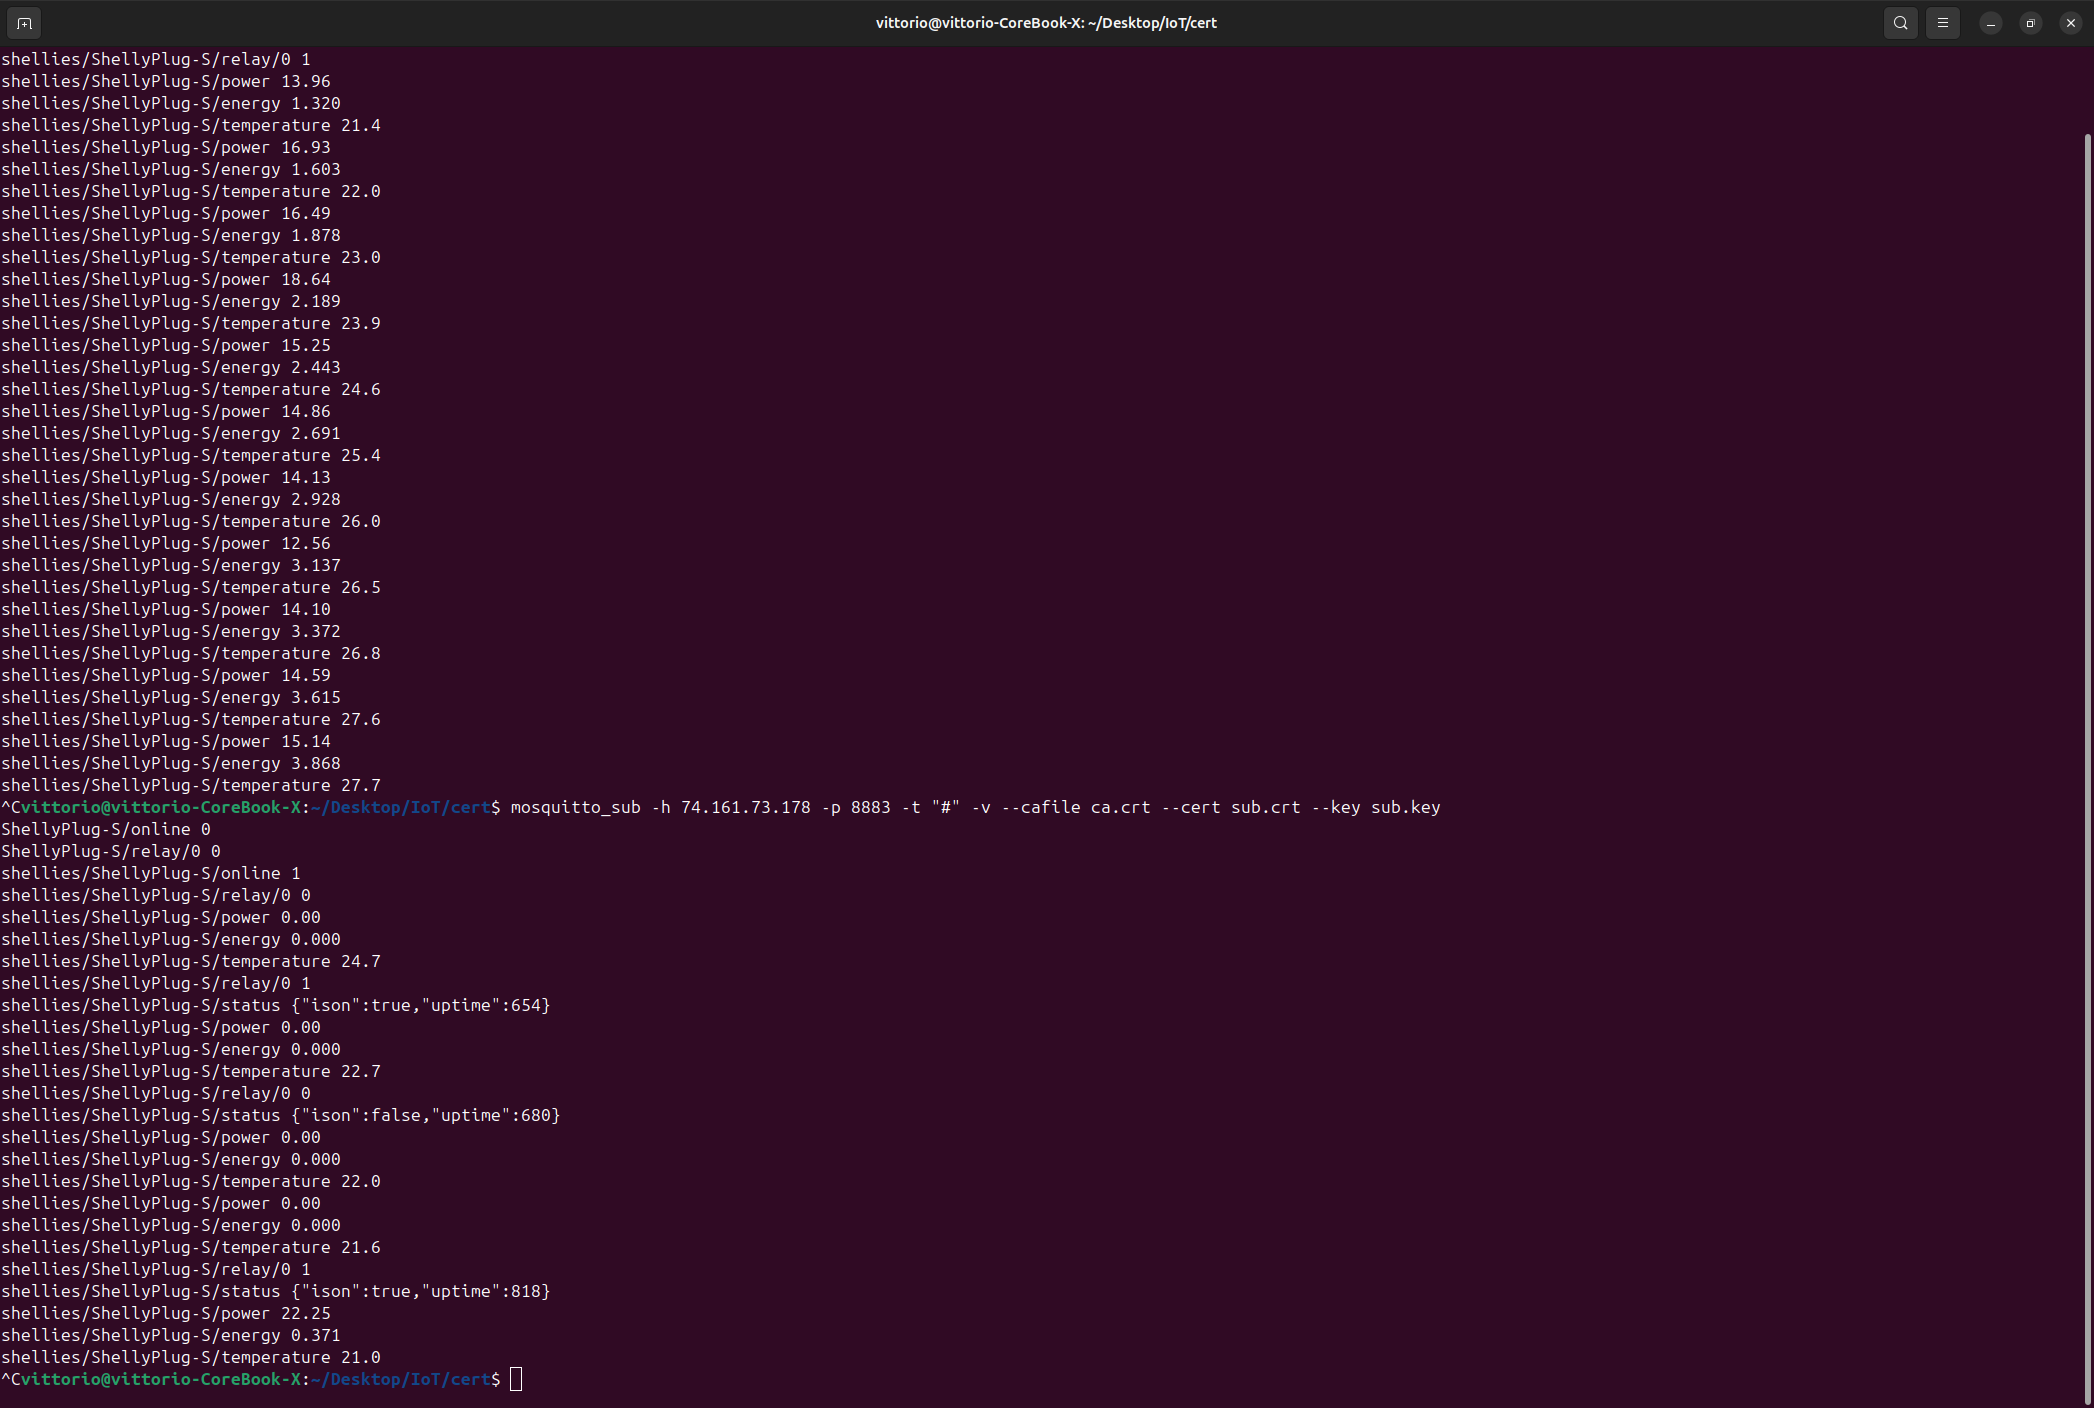
\includegraphics[width=0.95\linewidth]{Images/Fase3/MosquittoMQTTS2.png}
    \caption{Extended MQTTS session showing relay status changes and continuous telemetry from the Shelly device}
    \label{fig:mosquitto_sub_mqtts2}
\end{figure}

\subsubsection{Wireshark Verification: Encrypted Traffic}

To confirm that the MQTTS implementation effectively prevents traffic interception, a Wireshark capture was performed on the network. Figures~\ref{fig:wire_mqtts}--\ref{fig:wire_mqtts3} show the captured packets:

\begin{figure}[H]
    \centering
    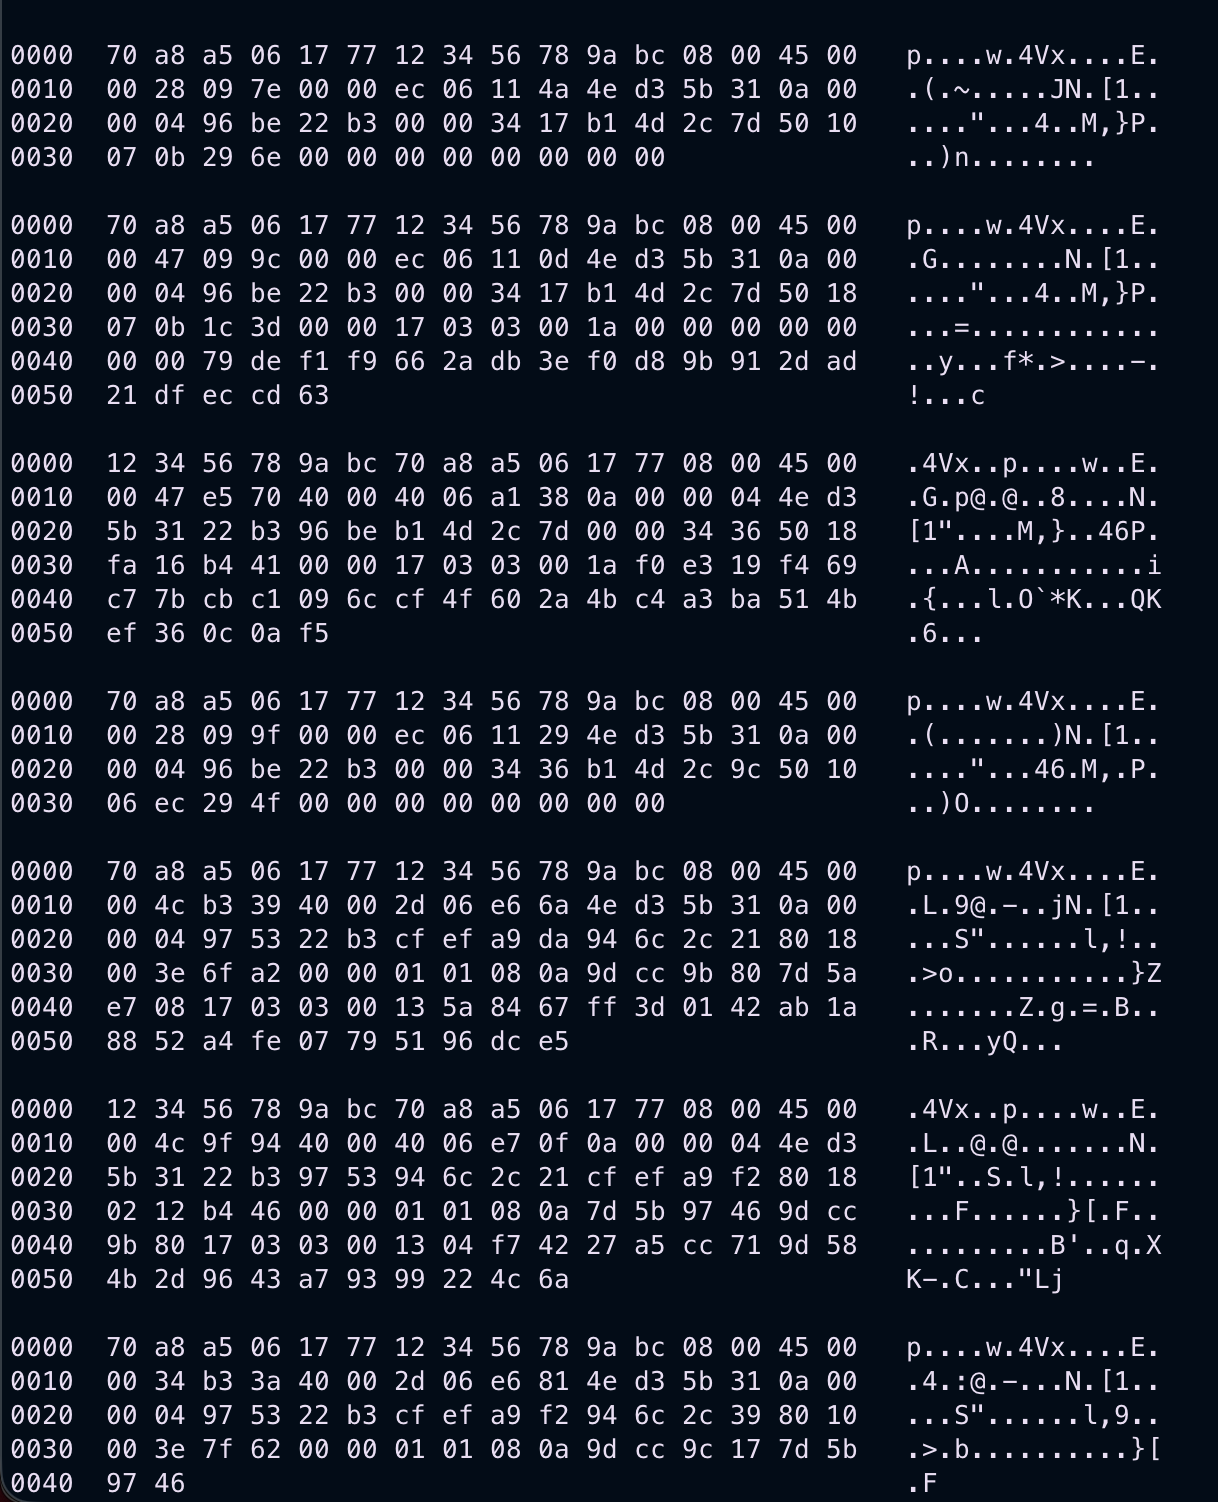
\includegraphics[width=0.95\linewidth]{Images/Fase3/WireMQTTS.png}
    \caption{Wireshark capture of MQTTS traffic: unlike Phase~1 where MQTT topics and payloads were visible in plaintext, all data is now encrypted and appears only as opaque ``Application Data'' on port 8883}
    \label{fig:wire_mqtts}
\end{figure}

\begin{figure}[H]
    \centering
    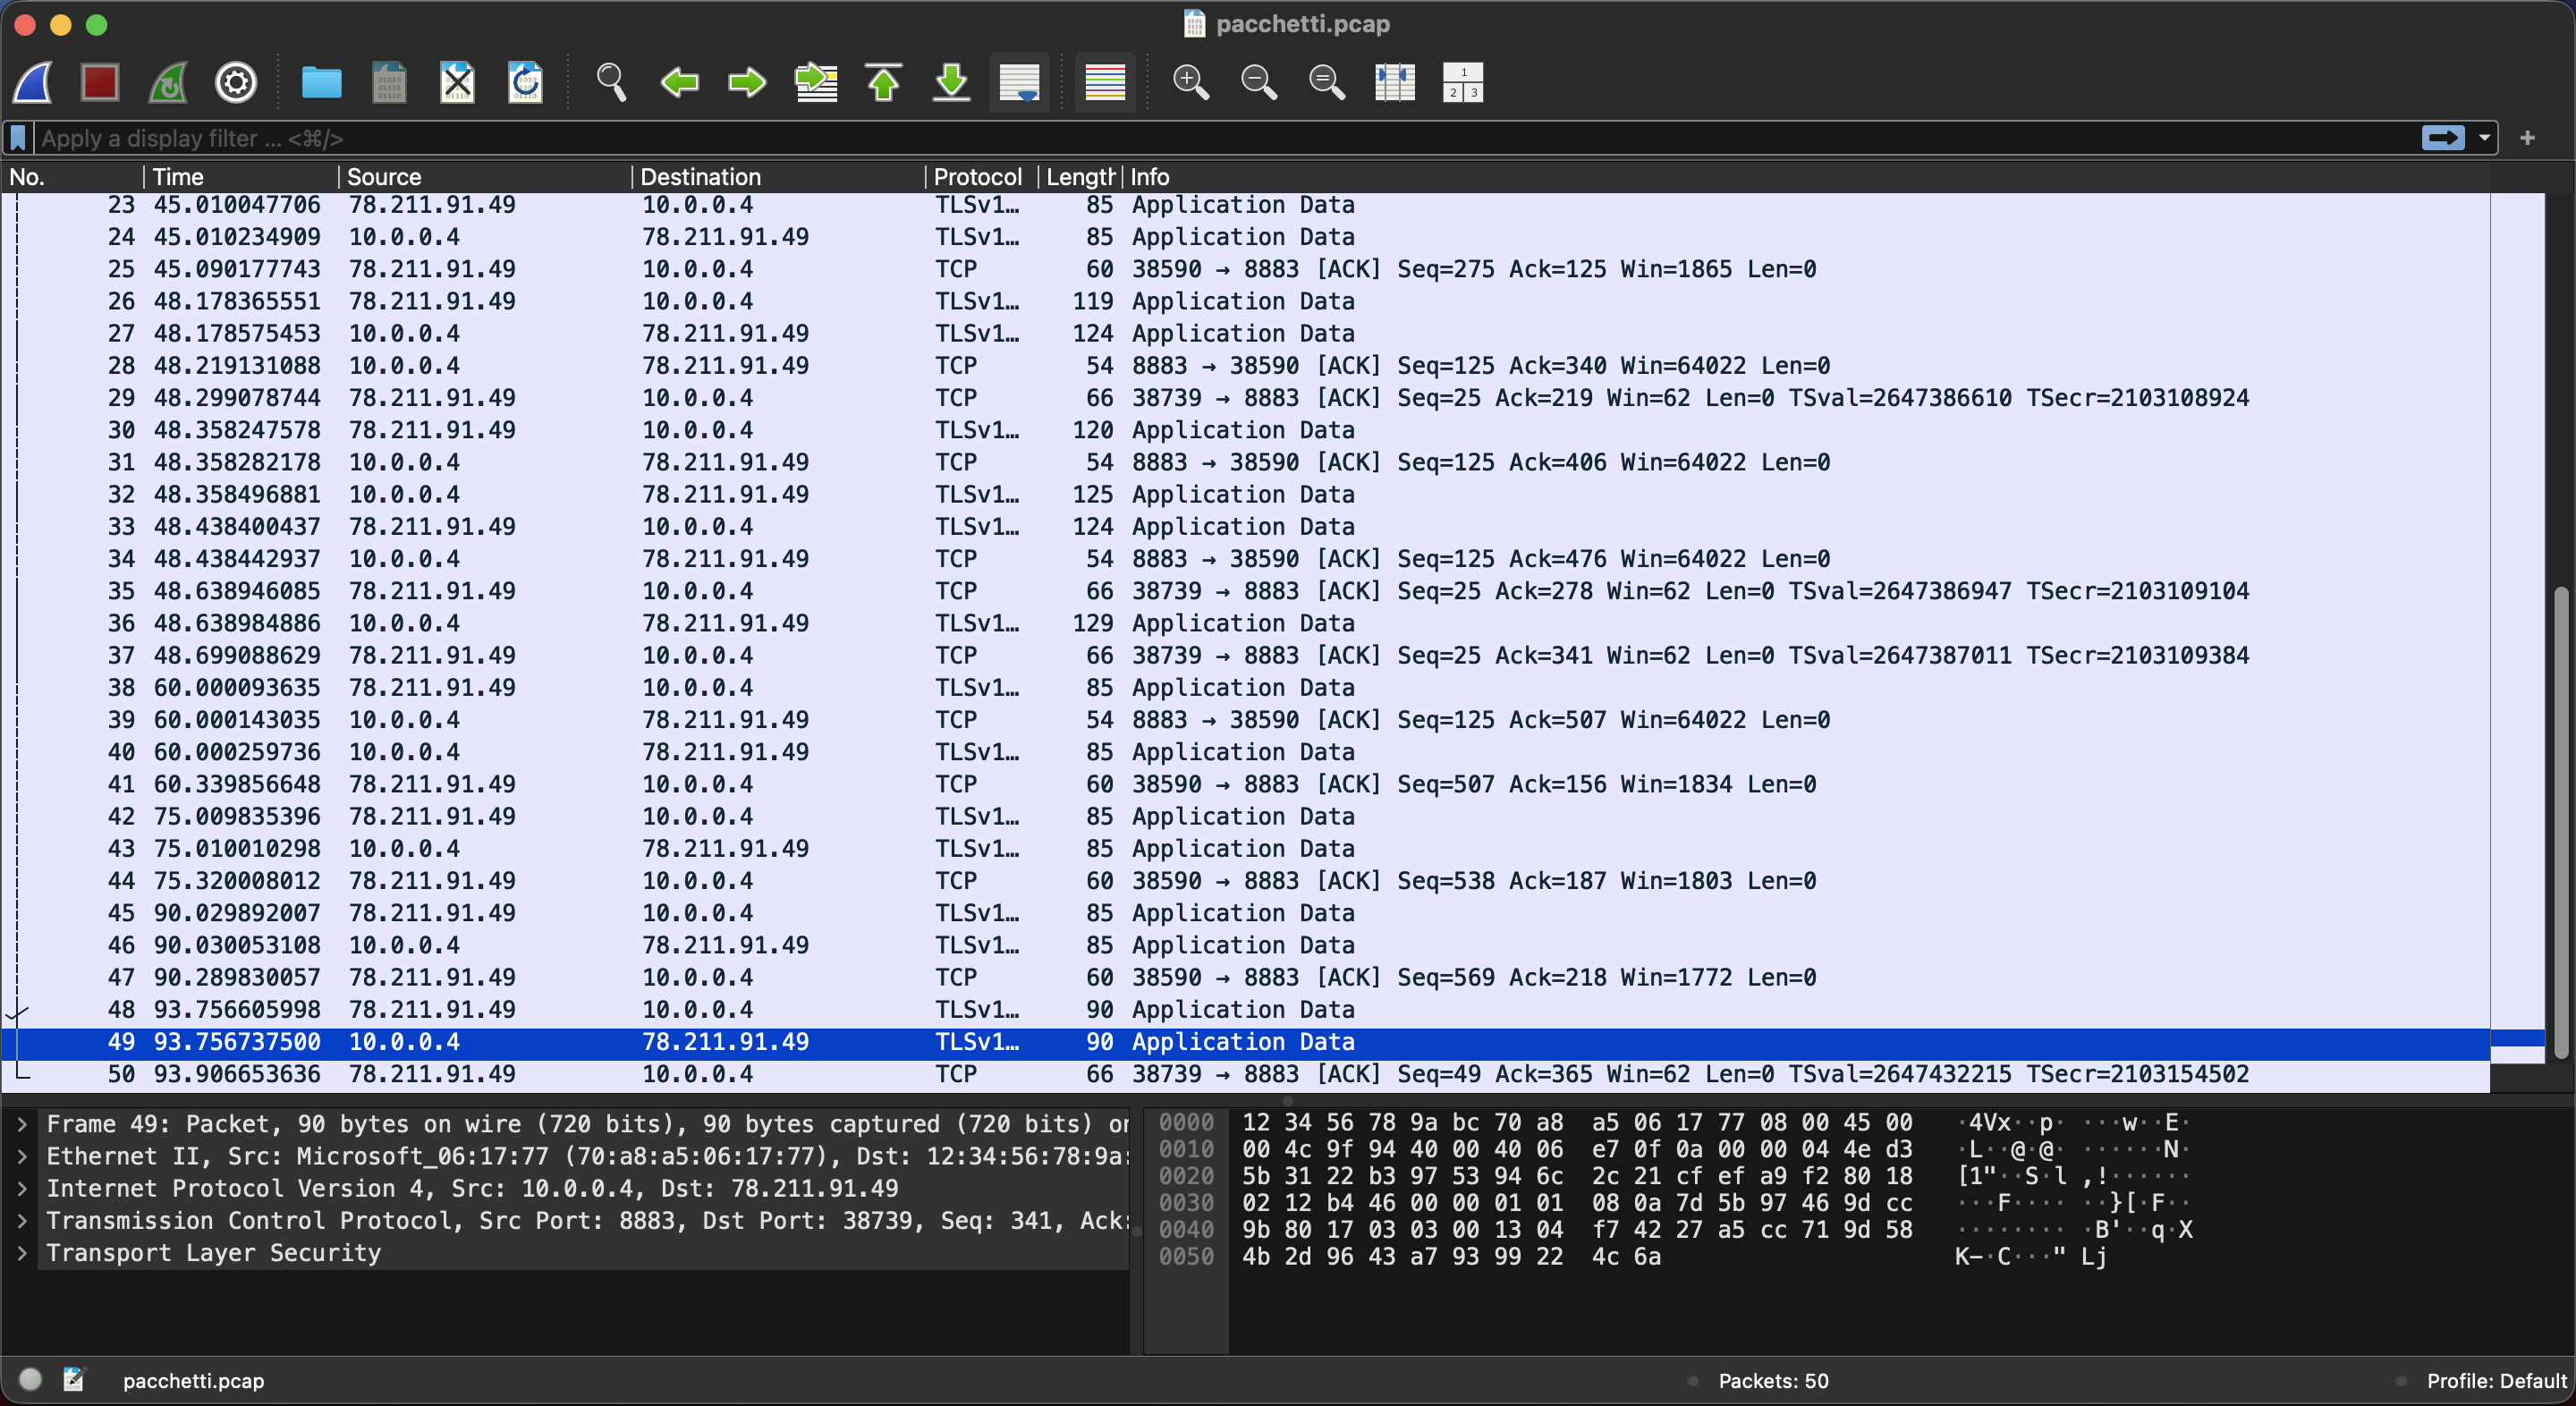
\includegraphics[width=0.95\linewidth]{Images/Fase3/WireMQTTS2.png}
    \caption{Detailed Wireshark view: the hex dump confirms that the TLS-encrypted payload is completely opaque — no MQTT topic names, power values, or relay states are visible in the captured data}
    \label{fig:wire_mqtts2}
\end{figure}

\begin{figure}[H]
    \centering
    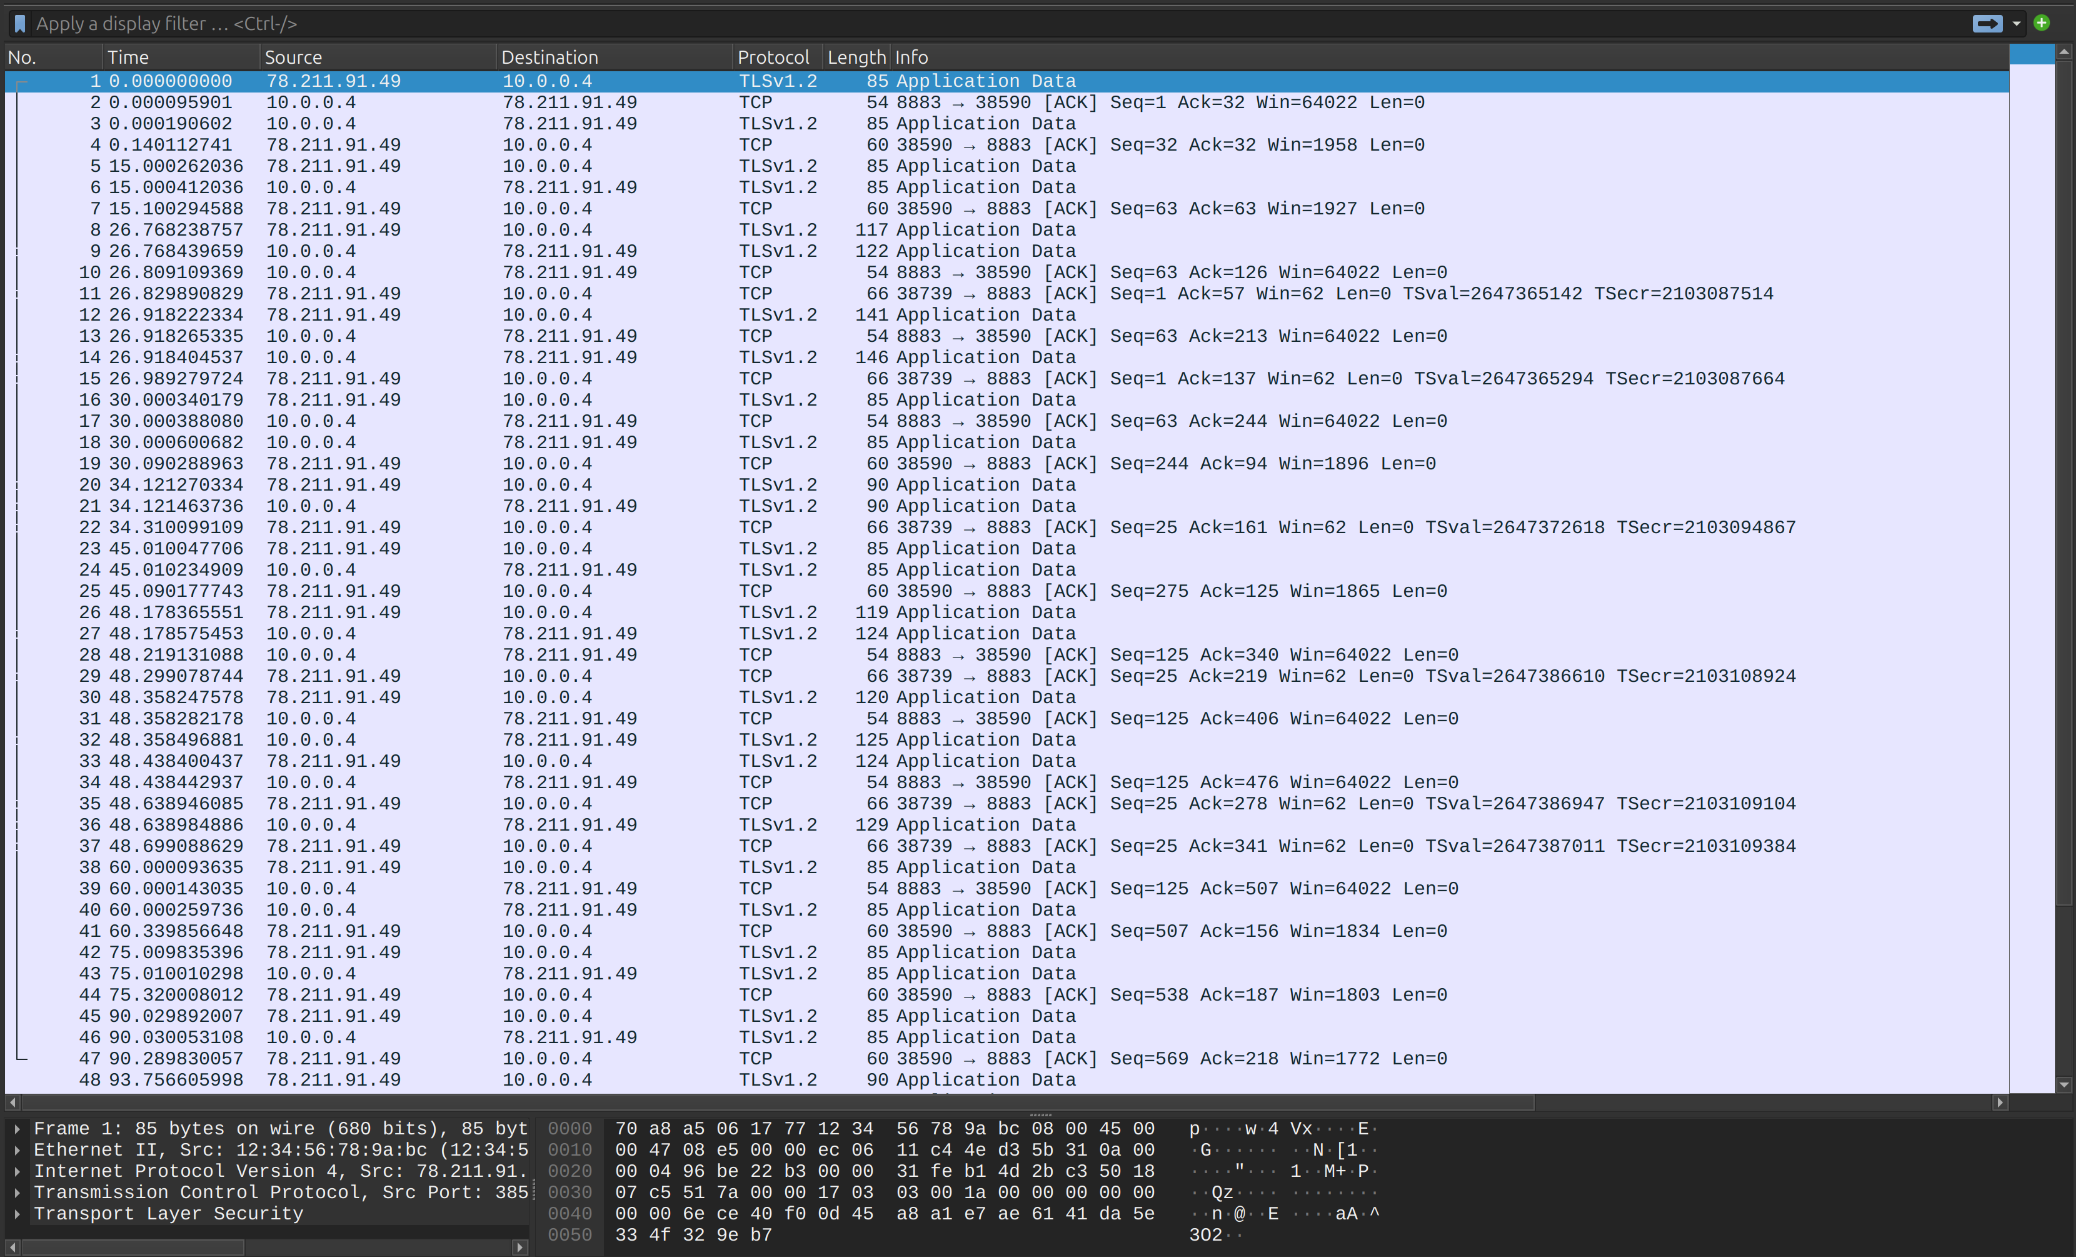
\includegraphics[width=0.95\linewidth]{Images/Fase3/WireMQTTS3.png}
    \caption{Full Wireshark session overview: all communication between the device and the broker is classified as TLSv1.2 ``Application Data'', with no readable MQTT content exposed at the network layer}
    \label{fig:wire_mqtts3}
\end{figure}

\noindent The Wireshark analysis conclusively demonstrates the effectiveness of the MQTTS countermeasure:

\begin{itemize}
    \item \textbf{Protocol}: All packets are classified as \texttt{TLSv1.2} instead of \texttt{MQTT}.
    \item \textbf{Port}: Communication occurs on port \texttt{8883} (MQTTS) instead of \texttt{1883} (MQTT).
    \item \textbf{Payload}: The hex dump shows only encrypted ``Application Data'', with no readable MQTT topic names (\texttt{shellies/...}), power values, or relay states visible. In contrast, the Phase~1 Wireshark captures showed all telemetry data in plaintext.
    \item \textbf{Mutual Authentication}: Without a valid client certificate signed by the CA, no entity can connect to the broker or intercept the communication, even if they are on the same local network.
\end{itemize}

\noindent This combination of transport encryption and mutual authentication effectively neutralizes the eavesdropping and traffic manipulation threats demonstrated in Phase~1, while maintaining full backward compatibility with the standard Shelly MQTT topic structure for seamless integration with home automation platforms.
